\documentclass[compress,red,notes]{beamer}
% Useful for practice: %can use [notes] or [notes=only]
% Useful for large documents with lots of images: [draft]
\usepackage{etex} %helps when using lots of packages
\mode<presentation>

\usepackage{amsmath}
\usepackage{amsthm}

%%%%%%%%%%%%%%%%%%%%%%%%%%%%%%%%%%%%%%%%
                                       %
% change this line for portable code:  %
\newcommand*{\commonDir}{../../common/}%
\input{\commonDir preambleCommon}      %
                                       %
%%%%%%%%%%%%%%%%%%%%%%%%%%%%%%%%%%%%%%%%

\usepackage{listings}
\usepackage{atslistings}
\usepackage{media9}
\usepackage{epstopdf}

\captionsetup[figure]{labelformat=empty}

\graphicspath{{./figures}{../../falconBioinfo/figures/}%
{../../epistasisSameGeneArXiv/figures/}{../../thesis/figures/}}

\usetheme{Warsaw}
% other themes: AnnArbor, Antibes, Bergen, Berkeley, Berlin, Boadilla, boxes, CambridgeUS, Copenhagen, Darmstadt, default, Dresden, Frankfurt, Goettingen,
% Hannover, Ilmenau, JuanLesPins, Luebeck, Madrid, Maloe, Marburg, Montpellier, PaloAlto, Pittsburg, Rochester, Singapore, Szeged, classic

%\usecolortheme{lily}
% color themes: albatross, beaver, beetle, crane, default, dolphin, dov, fly, lily, orchid, rose, seagull, seahorse, sidebartab, structure, whale, wolverine

%\usefonttheme{serif}
% font themes: default, professionalfonts, serif, structurebold, structureitalicserif, structuresmallcapsserif

\hypersetup{pdfpagemode=FullScreen} % makes your presentation go automatically to full screen

% define your own colors:
\definecolor{CURed}{rgb}{0.702,0.106,0.106}
\definecolor{CUGrey}{rgb}{0.302,0.31,0.3255}
%
\definecolor{White}{rgb}{1,1,1}
\definecolor{Red}{rgb}{1,0,0}
\definecolor{Blue}{rgb}{0,0,1}
\definecolor{Green}{rgb}{0,1,0}
\definecolor{magenta}{rgb}{1,0,.6}
\definecolor{lightblue}{rgb}{0,.5,1}
\definecolor{lightpurple}{rgb}{.6,.4,1}
\definecolor{gold}{rgb}{.6,.5,0}
\definecolor{orange}{rgb}{1,0.4,0}
\definecolor{hotpink}{rgb}{1,0,0.5}
\definecolor{newcolor2}{rgb}{.5,.3,.5}
\definecolor{newcolor}{rgb}{0,.3,1}
\definecolor{newcolor3}{rgb}{1,0,.35}
\definecolor{darkgreen1}{rgb}{0, .35, 0}
\definecolor{darkgreen}{rgb}{0, .6, 0}
\definecolor{darkred}{rgb}{.75,0,0}

\xdefinecolor{olive}{cmyk}{0.64,0,0.95,0.4}
\xdefinecolor{purpleish}{cmyk}{0.75,0.75,0,0}

% can also choose different themes for the "inside" and "outside"

% \usepackage{beamerinnertheme_______}
% inner themes include circles, default, inmargin, rectangles, rounded

% \usepackage{beamerouterthemesmoothbars}
% outer themes include default, infolines, miniframes, shadow, sidebar, smoothbars, smoothtree, split, tree

\useoutertheme[subsection=false]{smoothbars}

% to have the same footer on all slides
%\setbeamertemplate{footline}[text line]{STUFF HERE!}
\setbeamertemplate{footline}[text line]{} % makes the footer EMPTY

% Change some colors:
\setbeamercolor{structure}{fg=CURed}
\setbeamercolor*{palette quaternary}{fg=white,bg=CUGrey}

% include packages
\usepackage{multicol}
\usepackage{epsfig}
\usepackage[all,knot]{xy}
\xyoption{arc}
\usepackage{url}
\usepackage{hyperref}
     
%%%%%%%%%%%%%%%%%%%%%%%%%%%%%%%%%%%%%%%%%%%%%%%%%%%%%%%%%%%%%%%%%%%%%%%%%%%%%%%%%%%%%%%%%%
%%%%%%%%%%%%%%%%%%%%%%%%%%%%%% Title Page Info %%%%%%%%%%%%%%%%%%%%%%%%%%%%%%%%%%%%%%%%%%%
%%%%%%%%%%%%%%%%%%%%%%%%%%%%%%%%%%%%%%%%%%%%%%%%%%%%%%%%%%%%%%%%%%%%%%%%%%%%%%%%%%%%%%%%%%

\title{An Efficient Systems Approach to Whole-Cell Modeling}
%\subtitle{With a View}
\author{\texorpdfstring{Brandon Barker\newline
  \url{brandon.barker@gmail.com}}{Brandon Barker}}
\institute{
Tri-Institutional Program in Computational Biology and Medicine\\ 
Gu Laboratory\\
Cornell University \\ \vspace{.25cm}CAC Job Search}
\date{\today}

%%%%%%%%%%%%%%%%%%%%%%%%%%%%%%%%%%%%%%%%%%%%%%%%%%%%%%%%%%%%%%%%%%%%%%%%%%%%%%%%%%%%%%%%%%
%%%%%%%%%%%%%%%%%%%%%%%%%%%%%% Begin Your Document %%%%%%%%%%%%%%%%%%%%%%%%%%%%%%%%%%%%%%%
%%%%%%%%%%%%%%%%%%%%%%%%%%%%%%%%%%%%%%%%%%%%%%%%%%%%%%%%%%%%%%%%%%%%%%%%%%%%%%%%%%%%%%%%%%


\begin{document}

%%%%%%%%%%%%%%%%%%%%%%%%%%%%%%%%%%%%%%%%
                                       %
\newboolean{thesisStyle}               %
\setboolean{thesisStyle}{true}         %
                                       %
\input{\commonDir documentHeadCommon}  %
                                       %
%%%%%%%%%%%%%%%%%%%%%%%%%%%%%%%%%%%%%%%%

%\newcommand\Small{\fontsize{9}{9.2}\selectfont}
%\newcommand*\LSTfont{\scriptsize\ttfamily\SetTracking{encoding=*}{-60}\lsstyle}

%%%%%%%%%%%%%%%%%%%%%%%%%%%%%%%%%%%%%%%%%%%%%%%%%%%%%%%%%%%%%%%%%%%%%%%%%%%%%%%%%%%%%%%%%%

\frame{
  \titlepage 
}

%%%%%%%%%%%%%%%%%%%%%%%%%%%%%%%%%%%%%%%%%%%%%%%%%%%%%%%%%%%%%%%%%%%%%%%%%%%%%%%%%%%%%%%%%%
% this puts the outline before EACH section automatically & will
% highlight the section you're about to talk about
%\section[Outline]{}
%\frame{\tableofcontents}

%%%%%%%%%%%%%%%%%%%%%%%%%%%%%%%%%%%%%%%%%%%%%%%%%%%%%%%%%%%%%%%%%%%%%%%%%%%%%%%%%%%%%%%%%%


%%%%%%%%%%%%%%%%%%%%%%%%%
                        %
\section{Introduction}  %
\subsection{GPR rules}  %
                        %
%%%%%%%%%%%%%%%%%%%%%%%%%

%%%%%%%%%%%%%%%%%%%%%%%%%%%%%%%%%%%%%%%%%%%%%%%%%%%%%%%%%%%%%%%%%%%%%%%%%%%%%%%%%%%%%%%%%%

\note{Metabolism is critical for understanding wide classes of
diseases including diabetes, cancer, and inborn errors in metabolism.
Bio-energy and industrial bio-synthetics are inherently tied to the
engineering of robust and novel metabolic networks. Metabolism is also
beginning to provide fine-grained detail to understanding microbial
ecologies. One way to describe metabolism is as the set of reactions
and the rate of the reactions made possible by enzymatic catalysts.
Here we can see several very important reactions that organisms from
yeasts to humans require, the ultimate step being the generation of
ATP by this motor-like enzyme complex called ATP Synthase. We'll come
back to ATP synthase in a later example.

Unfortunately, metabolism is much more complex than is often
depicted. This depiction only shows a little over half of what would
be considered a fairly typical length for a pathway.  This pathway is
inherently linked to another pathway of about the same size, and that
pathway depends on another core pathway of roughly the same length for
preprocessing glucose. When we zoom out, we can start to see some of
this complexity.}

\frame{\frametitle{Important metabolic pathways}
\begin{center}
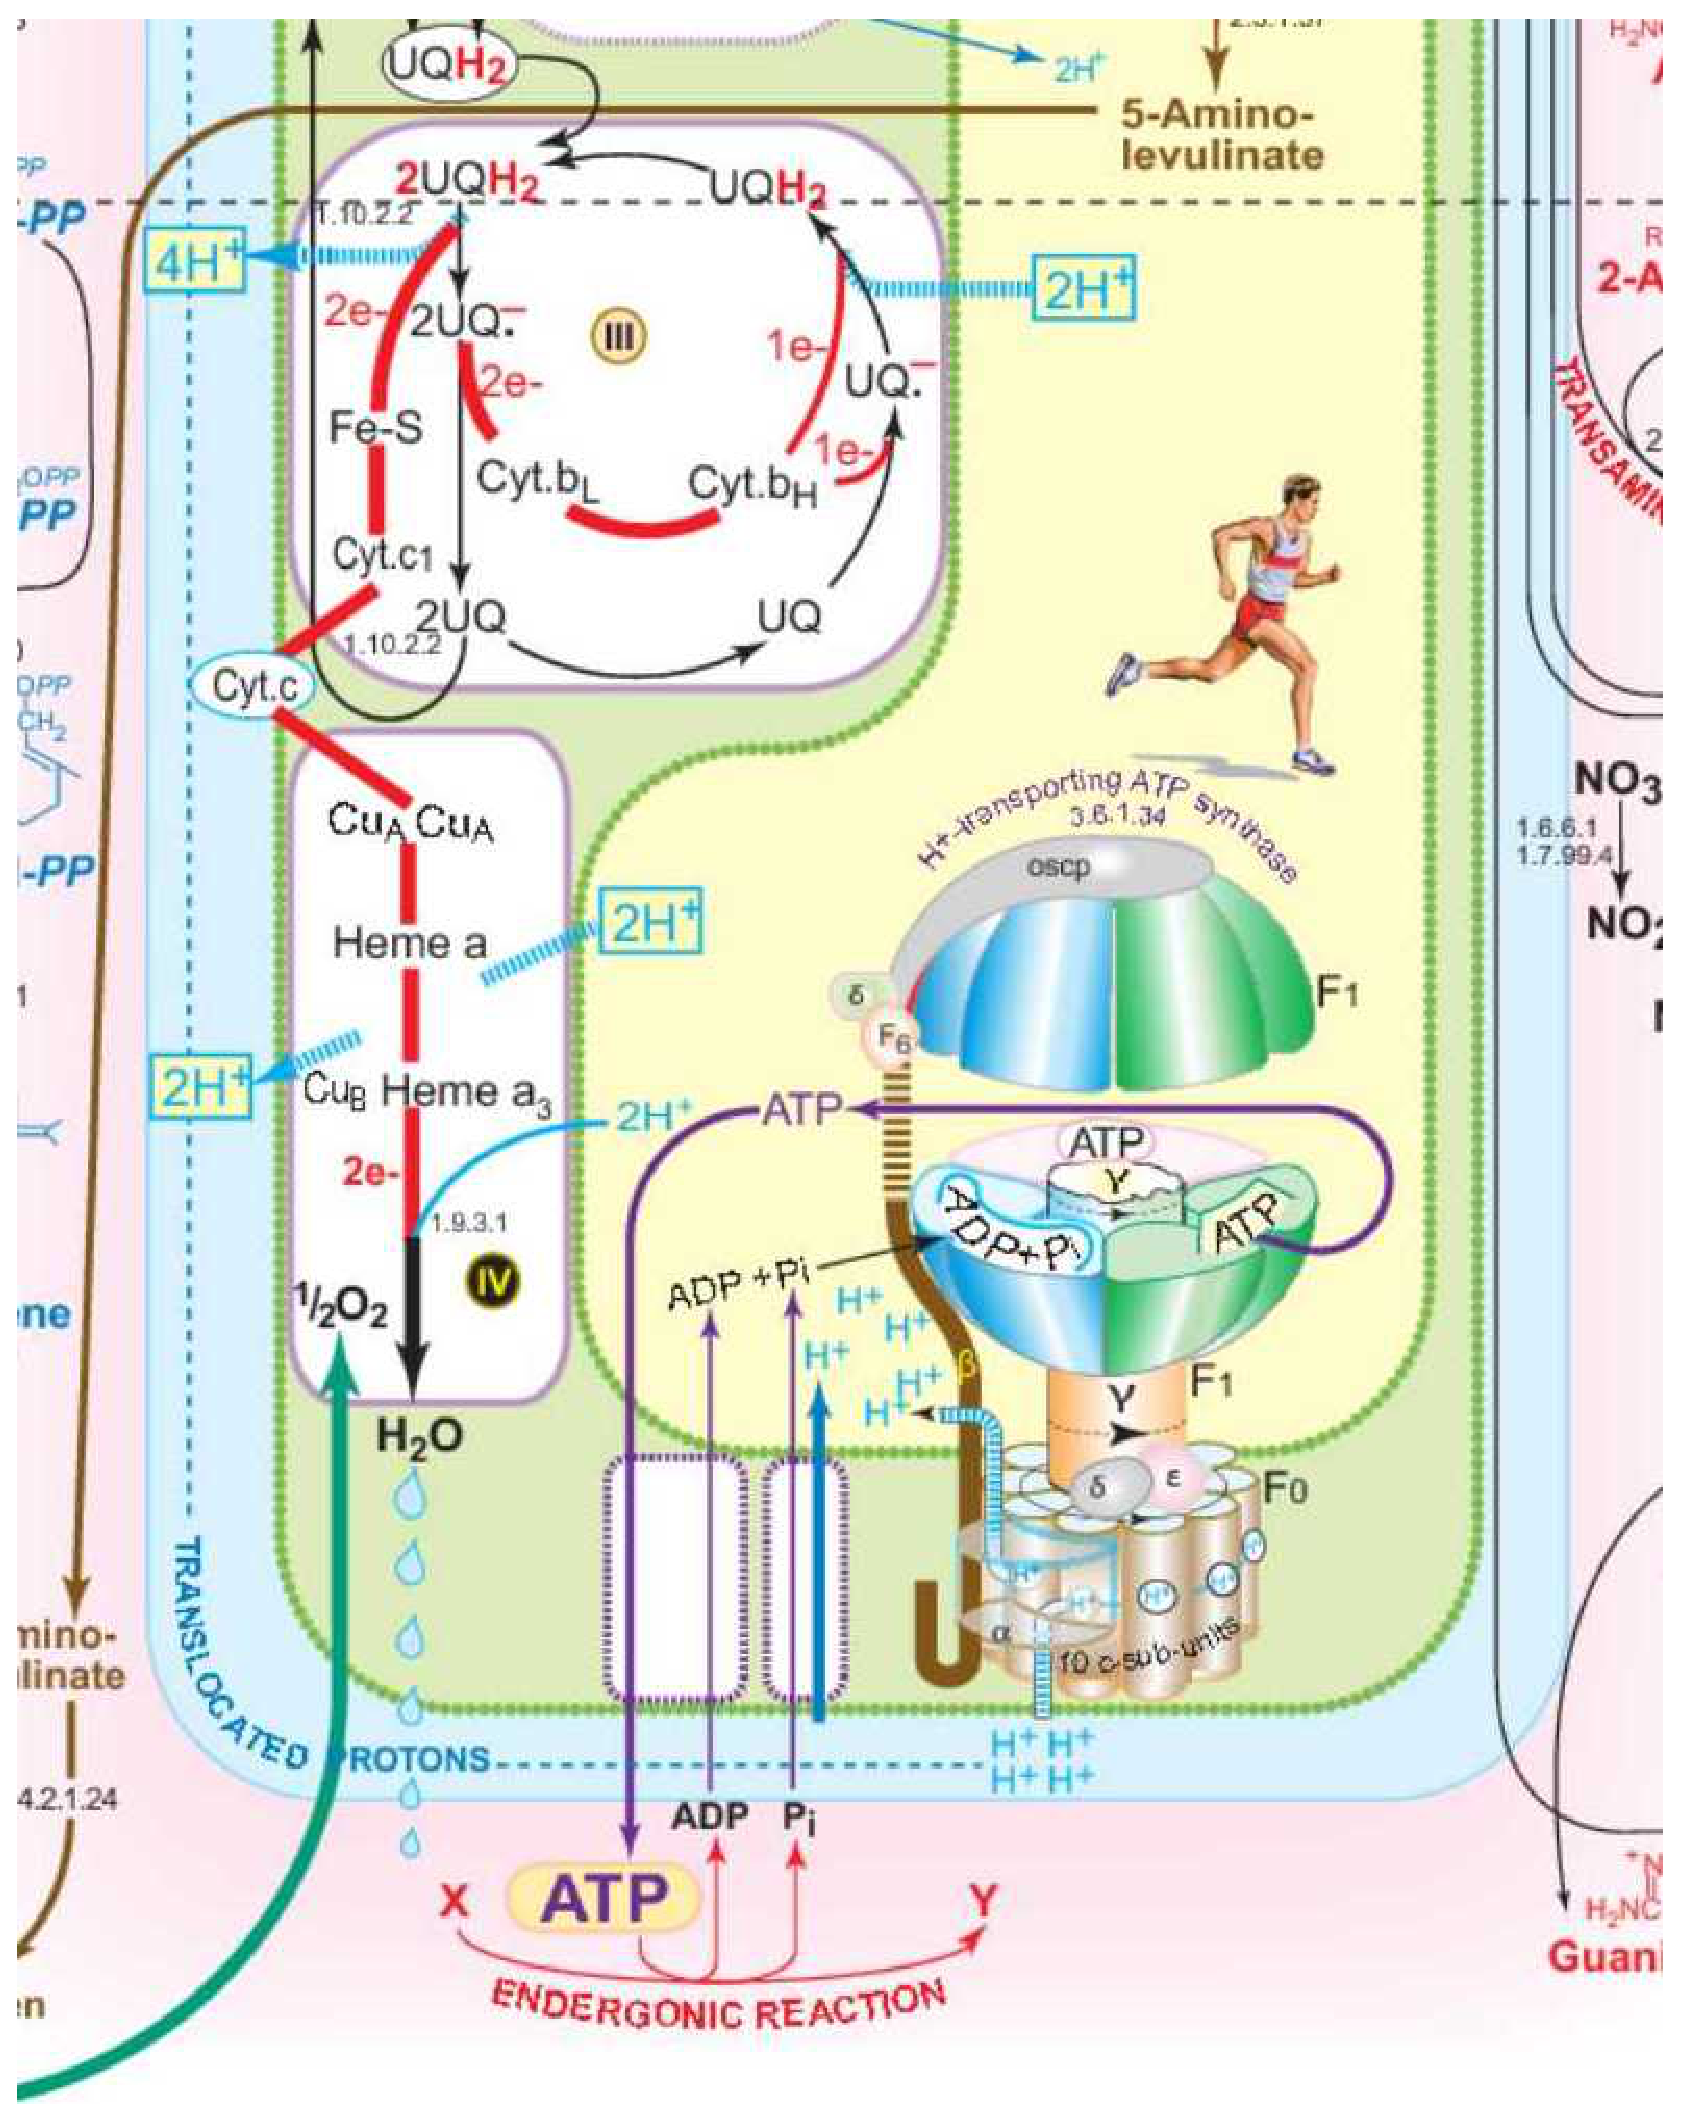
\includegraphics[height=0.85\textheight,width=0.53\textwidth]
{./figures/metabolism-zoom-start}
\end{center}
}
%
%

\note{Here you can see the rest of the first pathway, oxidative
phosphorylation, and its sister pathway, the TCA cycle. And this
little linear pathway is glycolysis, which converts glucose into a
usable form for the TCA cycle. In practice, these pathways also
require many other pathway dependencies that process or recycle other
chemicals that are not quite in the right form to be used by the later
stages. What's more, this poster from 2003 is actually relatively
simple: chemicals that are similar are often omitted, and there can be
thousands of these for some classes. Also, reactions are present but
are thought to be unimportant often are not drawn. }
\frame{\frametitle{Important metabolic pathways}
\begin{center}
\includemedia[
  activate=pageopen,
  height=0.85\textheight,
  width=0.53\textwidth,
  transparent=true
]
{}{./figures/metabolism-zoom.swf}
\end{center}
}

%%%%%%%%%%%%%%%%%%%%%%%%%%%%%%%%%%%%%%%%%%%%%%%%%%%%%%%%%%%%%%%%%%%%%%%%%%%%%%%%%%%%%%%%%%

\note{
Talk about how FBA is not always great.\\
}
\frame{\frametitle{An overview to constraint-based modeling}
\begin{columns}
\begin{column}{0.5\textwidth}
\includegraphics[width=\textwidth, bb=13 730 671 1146, clip=true]
{SmatExample.eps}
\\
\includegraphics[width=\textwidth, bb=13 439 722 722, clip=true]
{SmatExample.eps}
\end{column}
\begin{column}{0.5\textwidth}
\includegraphics[width=\textwidth, bb= 13 13 722 435, clip=true]
{SmatExample.eps}
\end{column}

\end{columns}

}


%%%%%%%%%%%%%%%%%%%%%%%%%%%%%%%%%%%%%%%%%%%%%%%%%%%%%%%%%%%%%%%%%%%%%%%%%%%%%%%%%%%%%%%%%%

\frame{\frametitle{How did we get here? (change this? transition)}

\begin{block}{Flux fitting}
% Started as a way to fit a perturbed model to a wild-type flux.\\
Formulated as quadratic least-squares optimization (Segre et al 2002):\\
\begin{center}
$\textnormal{minimize}\ \sum\limits_{i=1}^N (v_i-a_i)^2$ 
\end{center}
Later formulated as a linear programing (LAD) variant.
\end{block}


\begin{block}{Expression-flux fitting}
A new way to constrain models.\\
Expression is widely available, especially for diseases\\
\hl{relevance to disease (Diabetes, Cancer, Drug discovery etc.)}

\end{block}

}

%%%%%%%%%%%%%%%%%%%%%%%%%%%%%%%%%%%%%%%%%%%%%%%%%%%%%%%%%%%%%%%%%%%%%%%%%%%%%%%%%%%%%%%%%%

%%%%%%%%%%%%%%%%%%%%
\section{Methods}  %
%%%%%%%%%%%%%%%%%%%%

%%%%%%%%%%%%%%%%%%%%%%%%%%%%%%%%%%%%%%%%%%%%%%%%%%%%%%%%%%%%%%%%%%%%%%%%%%%%%%%%%%%%%%%%%%
\frame{\frametitle{A popular enzyme complex.}

\begin{figure}
\centering
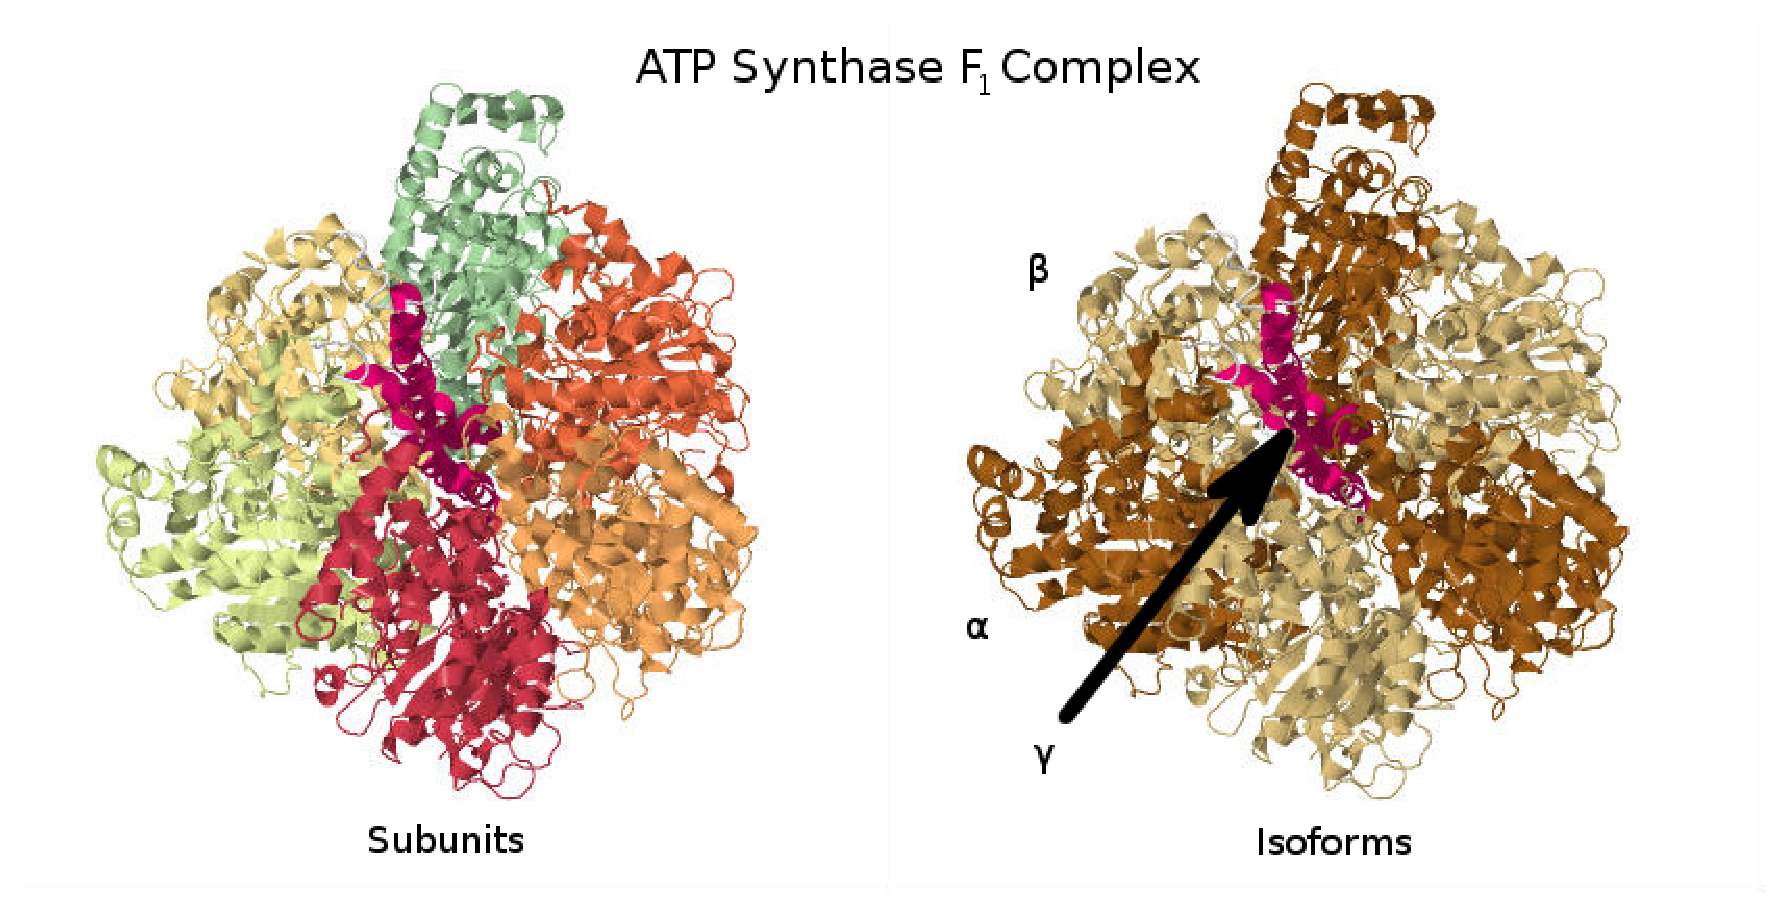
\includegraphics[clip=true,trim=0cm 0cm 0cm 0cm, width=6cm]{2F43}
\caption{Illustration of the $F_1$ part of the ATP Synthase complex
(PDB ID 1E79).}
\label{fig:2F43}
\end{figure}

}

%%%%%%%%%%%%%%%%%%%%%%%%%%%%%%%%%%%%%%%%%%%%%%%%%%%%%%%%%%%%%%%%%%%%%%%%%%%%%%%%%%%%%%%%%%

\frame{\frametitle{Equivalent GPR rules can be evaluated differently}

\begin{block}{Let's look at an example.}
For genes A, B, and C:\\
Rules $r_1$ and $r_2$ are equivalent logically.\\
However, they can be interpreted differently.
\end{block}

\begin{center}
\begin{tabular}{cccccccc}
$r_1$ & := & [A and B] or [A and C] & $\rightarrow$ & $e_1$  &=& $\min(a,b$) + $\min(a,c$) \\ 
$r_2$ & := & [A and (B or C)]       & $\rightarrow$ & $e_2$  &=&  $\min(a, b + c$) 
\end{tabular} 
\end{center}

}

%%%%%%%%%%%%%%%%%%%%%%%%%%%%%%%%%%%%%%%%%%%%%%%%%%%%%%%%%%%%%%%%%%%%%%%%%%%%%%%%%%%%%%%%%%

Put code adjacent to this.

\frame{
\frametitle{Flowchart illustrating the two algorithms in the pipeline.}
\hl{highlight algorithms}
\begin{figure}
\centering
\begin{tikzpicture}[scale=0.5, every node/.style={scale=0.5}]%[scale=0.8, node distance = 1cm, auto]
    % Place nodes
    \node [block] (start) {start}; 
    \node [iogram, below of=start, left of=start, xshift=-0.2cm] (exp) {Genes:\\ expression 
      ($\mu$,~$\sigma$)}; 
    \node [iogram, below of=start, right of=start] (rules) {Reactions:
      GPR Rule}; 
    \node [block, below of=rules] (parse) {Parse Rule}; 
    \node [block, below of=parse, left of=parse, xshift=-0.5cm]
      (mindisj) {Find minimum disjunction};
    \node [iogram, below of=mindisj] (expstd)
          {Reactions (enzyme~complexes):\\ abundance ($\mu$,~$\sigma$)};
    \node [iogram, right of=falcon, below of=expstd, xshift=0.2cm] (smat) 
      {$\mathbf{S}$ matrix};
    \node [iogram, left of=falcon, below of=expstd, xshift=-0.3cm] (vbnd) 
      {Reactions:\\ flux bounds ($\mathbf{v}_{lb}$, $\mathbf{v}_{ub}$)};
    \node [block, below of=vbnd, left of=smat, right of=vbnd, 
      below of=expstd, yshift=-0.5cm] (falcon) 
      {Flux fitting (FALCON)};
    \node [iogram, below of=falcon] (fluxout) 
      {Reactions:\\ fluxes ($\mathbf{v}:$ $\mu$,~$\sigma$)};
    % Draw edges
    \path [line] (start) -- (exp);
    \path [line] (start) -- (rules);
    \path [line] (rules) -- (parse);
    \path [line] (exp.south) -- (mindisj);
    \path [line] (parse) -- (mindisj);
    \path [line] (mindisj) -- (expstd);
    \path [line, transform canvas={xshift=0.1cm}] (expstd) -- (falcon);
    \path [line] (rules.east) |- (falcon.east);
    \path [line] (smat) -- (falcon);
    \path [line] (vbnd) -- (falcon);
    \path [line] (falcon) -- (fluxout);

\end{tikzpicture}
\end{figure}

}


%%%%%%%%%%%%%%%%%%%%%%%%%%%%%%%%%%%%%%%%%%%%%%%%%%%%%%%%%%%%%%%%%%%%%%%%%%%%%%%%%%%%%%%%%%

\begin{frame}[fragile]
\frametitle{GPR code (change title)}

Before this, put in an example showing actual GPR data
(and maybe other recon data) for human.

\begin{columns}
%
\begin{column}{0.5\textwidth}
\lstinputlisting[basicstyle=\ttfamily\tiny, language=ATS, showstringspaces=false]
{falcon_main_fun.dats}
\end{column}
%
\vrule{}
%
\begin{column}{0.5\textwidth}
\lstinputlisting[basicstyle=\ttfamily\tiny, language=ATS, showstringspaces=false]
{falcon_example.dats}
\end{column}
%
\end{columns}
\end{frame}

%%%%%%%%%%%%%%%%%%%%%%%%%%%%%%%%%%%%%%%%%%%%%%%%%%%%%%%%%%%%%%%%%%%%%%%%%%%%%%%%%%%%%%%%%%

\frame{\frametitle{Grouping reactions by enzyme complex has a large effect} 

\begin{figure}
\centering
\begin{tabular}{cc}
  \begin{subfigure}[b]{0.45\textwidth}
  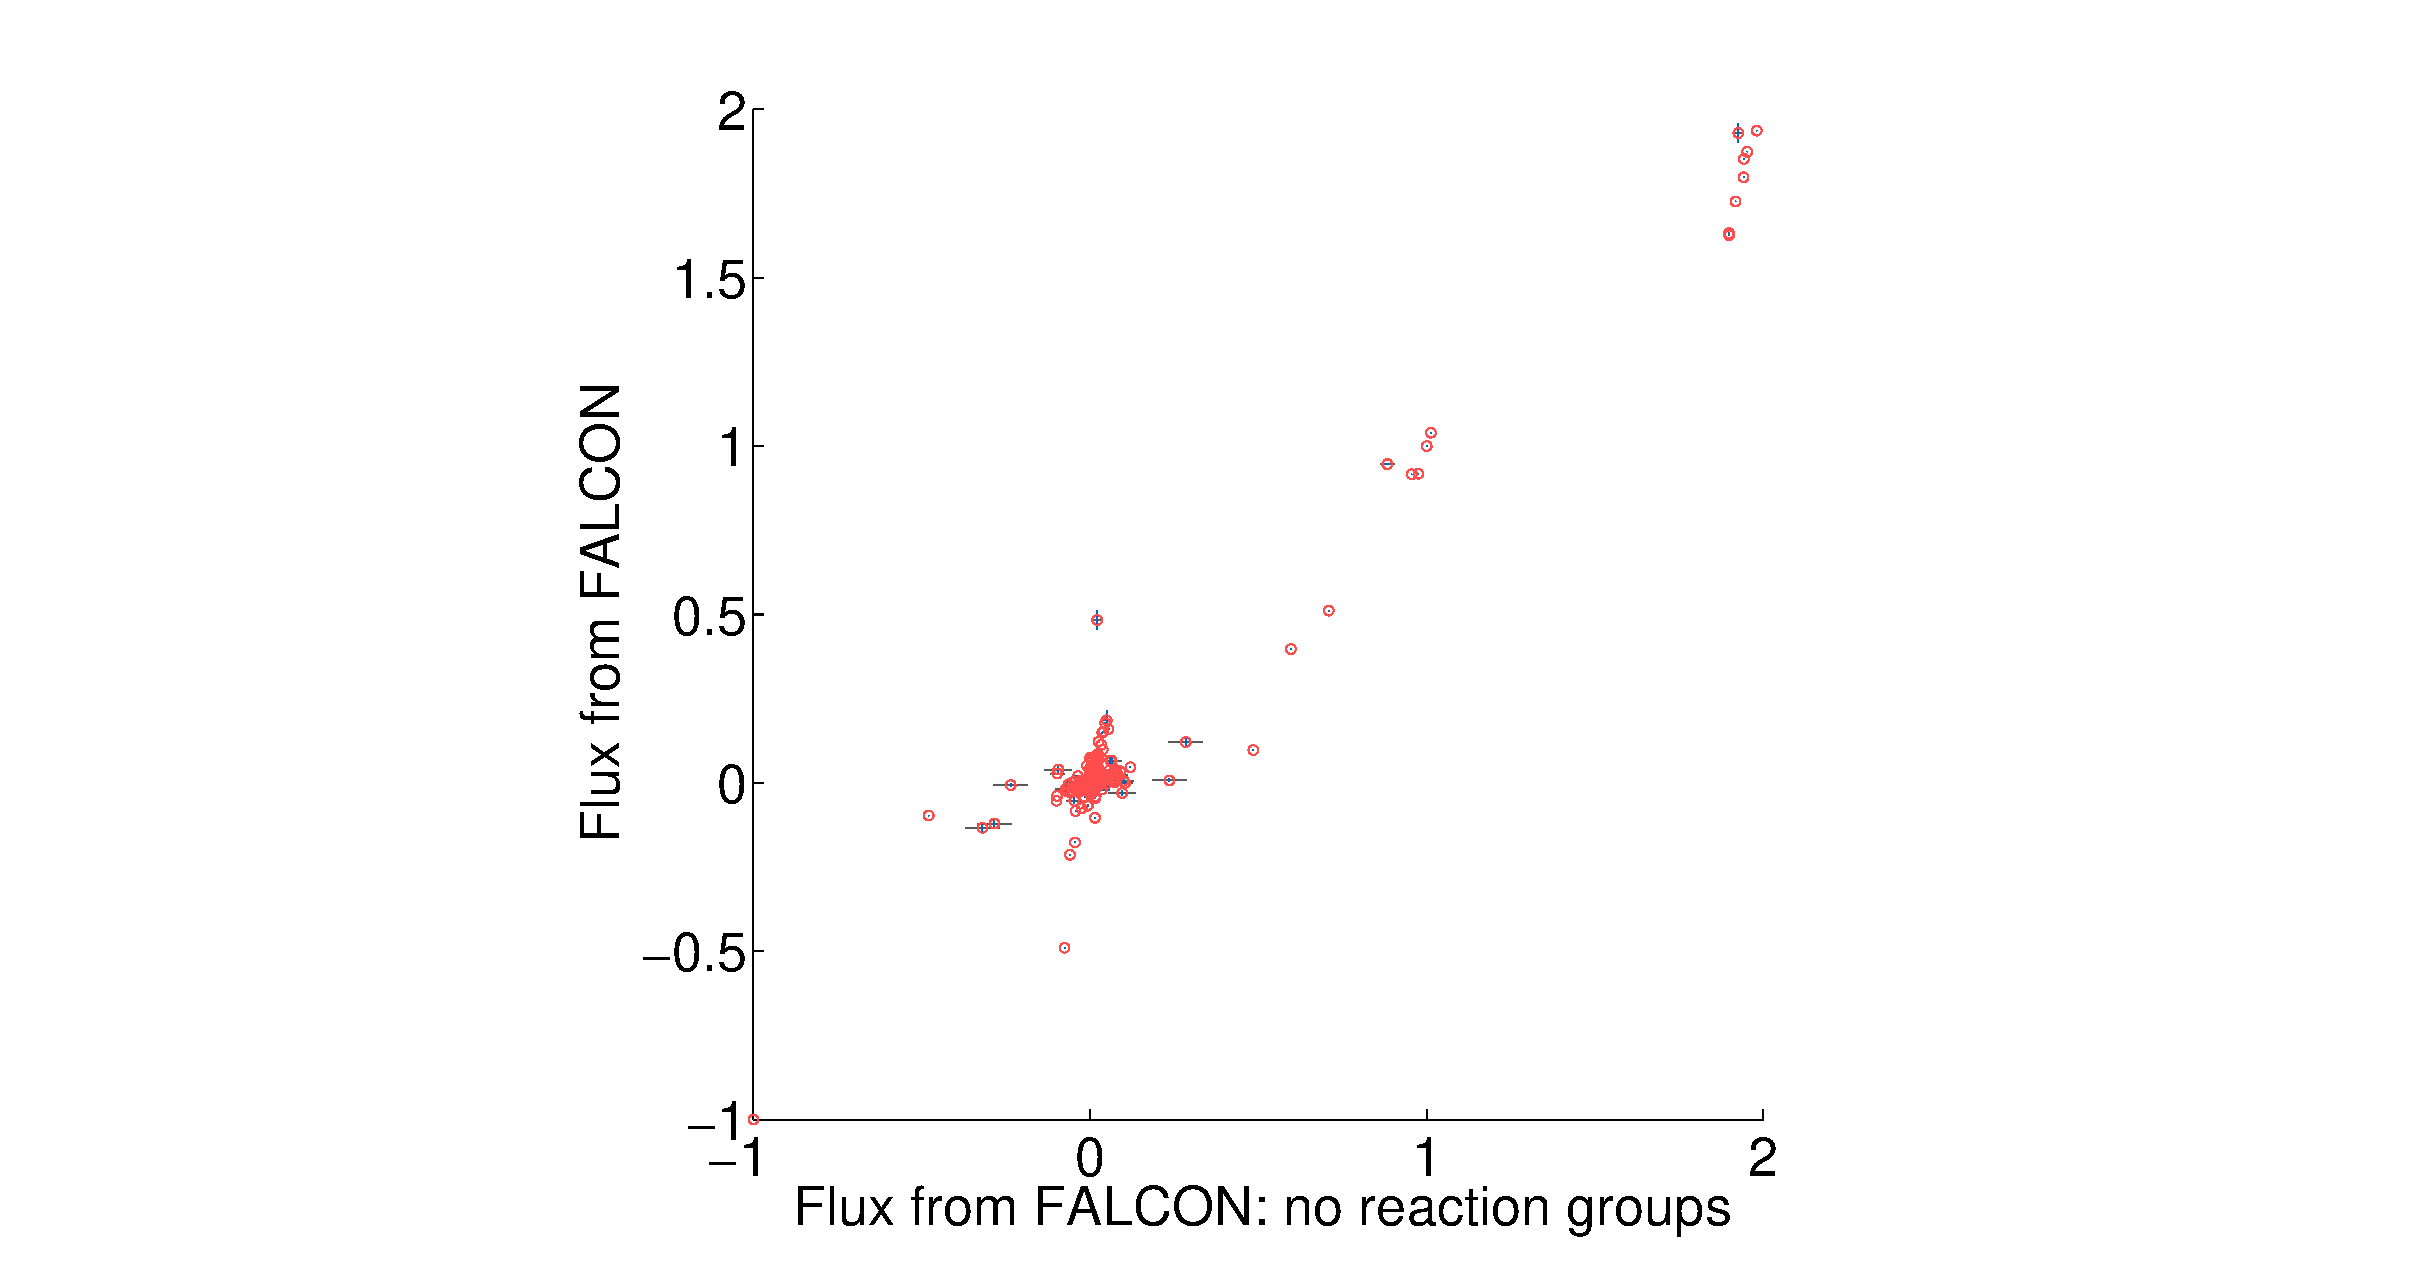
\includegraphics[width=\textwidth, trim=9cm 0cm 9cm 0cm, clip=true]
  {falconGrp_yeastHC}
  \caption{} \label{fig:FalconGrp:A}
  \end{subfigure}
&
  \begin{subfigure}[b]{0.45\textwidth}
  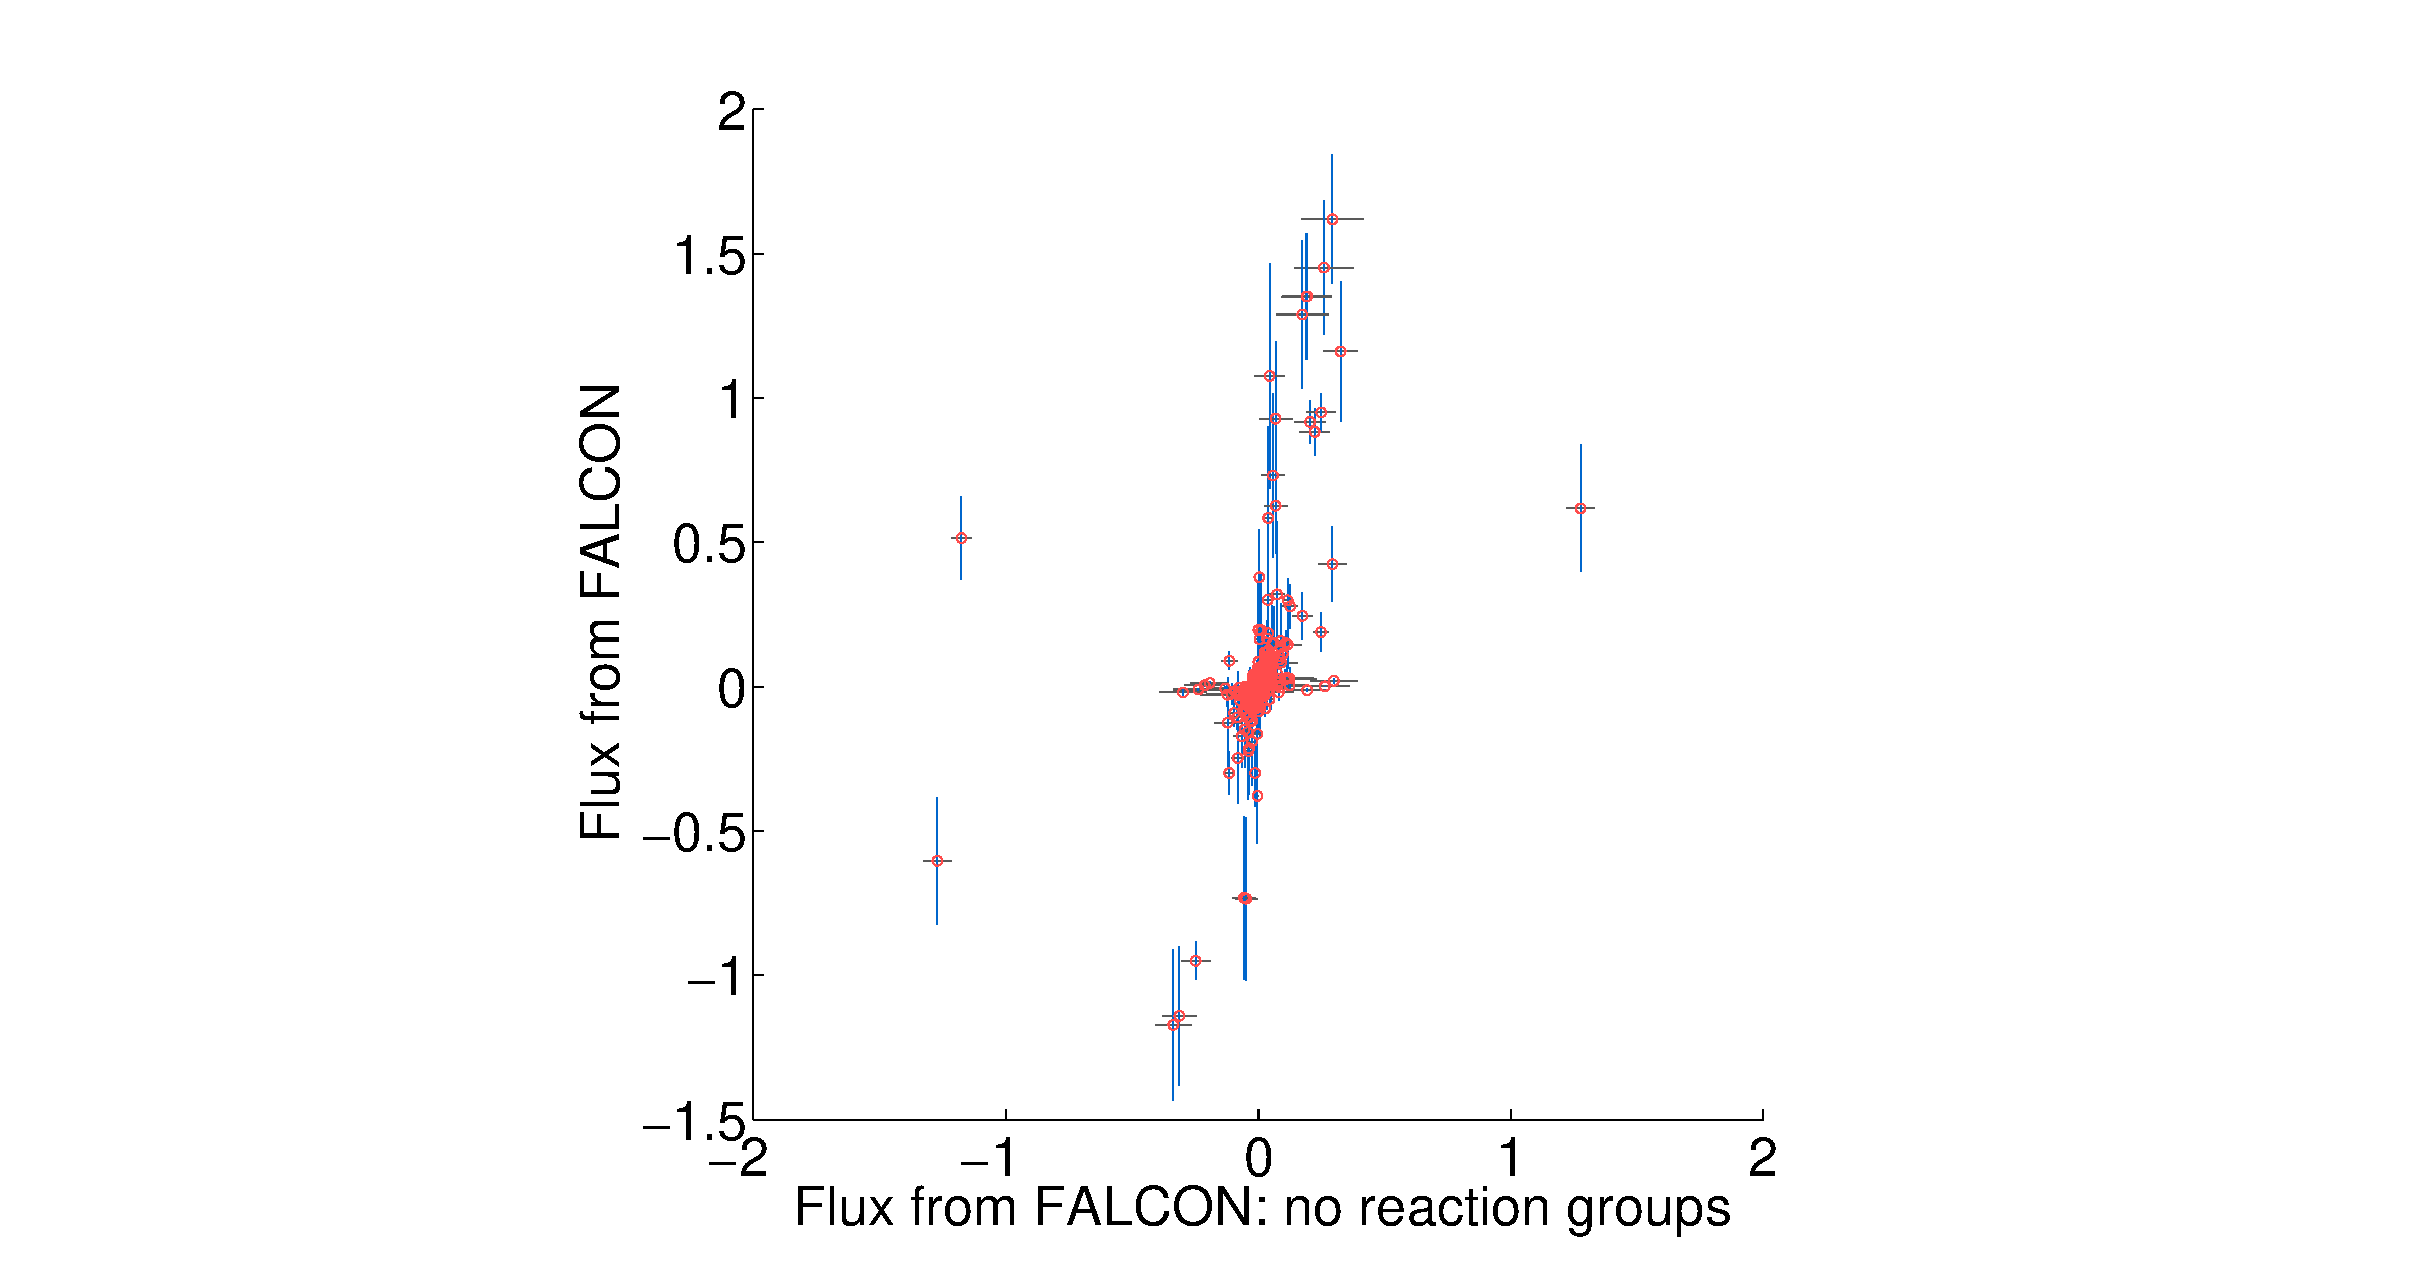
\includegraphics[width=\textwidth, trim=9cm 0cm 9cm 0cm, clip=true]
  {falconGrp_yeastMC}
  \caption{} \label{fig:FalconGrp:B}
  \end{subfigure} 
\\
\end{tabular}
\vspace{-4mm} 
\caption{
Comparison of setting FALCON to use no reaction group information (x-axis)
versus with group information (y-axis; default FALCON setting) with highly  
\textbf{(a)} and minimally \textbf{(b)} constrained models.}
\label{fig:FalconGrp}
\end{figure}
}


%%%%%%%%%%%%%%%%%%%%%%%%%%%%%%%%%%%%%%%%%%%%%%%%%%%%%%%%%%%%%%%%%%%%%%%%%%%%%%%%%%%%%%%%%%

Merge yeast and human slide.

\frame{\frametitle{Complexation effect in flux mapping: yeast} 

\begin{figure}
\centering
\begin{tabular}{cc}
  \begin{subfigure}[b]{0.5\textwidth}
  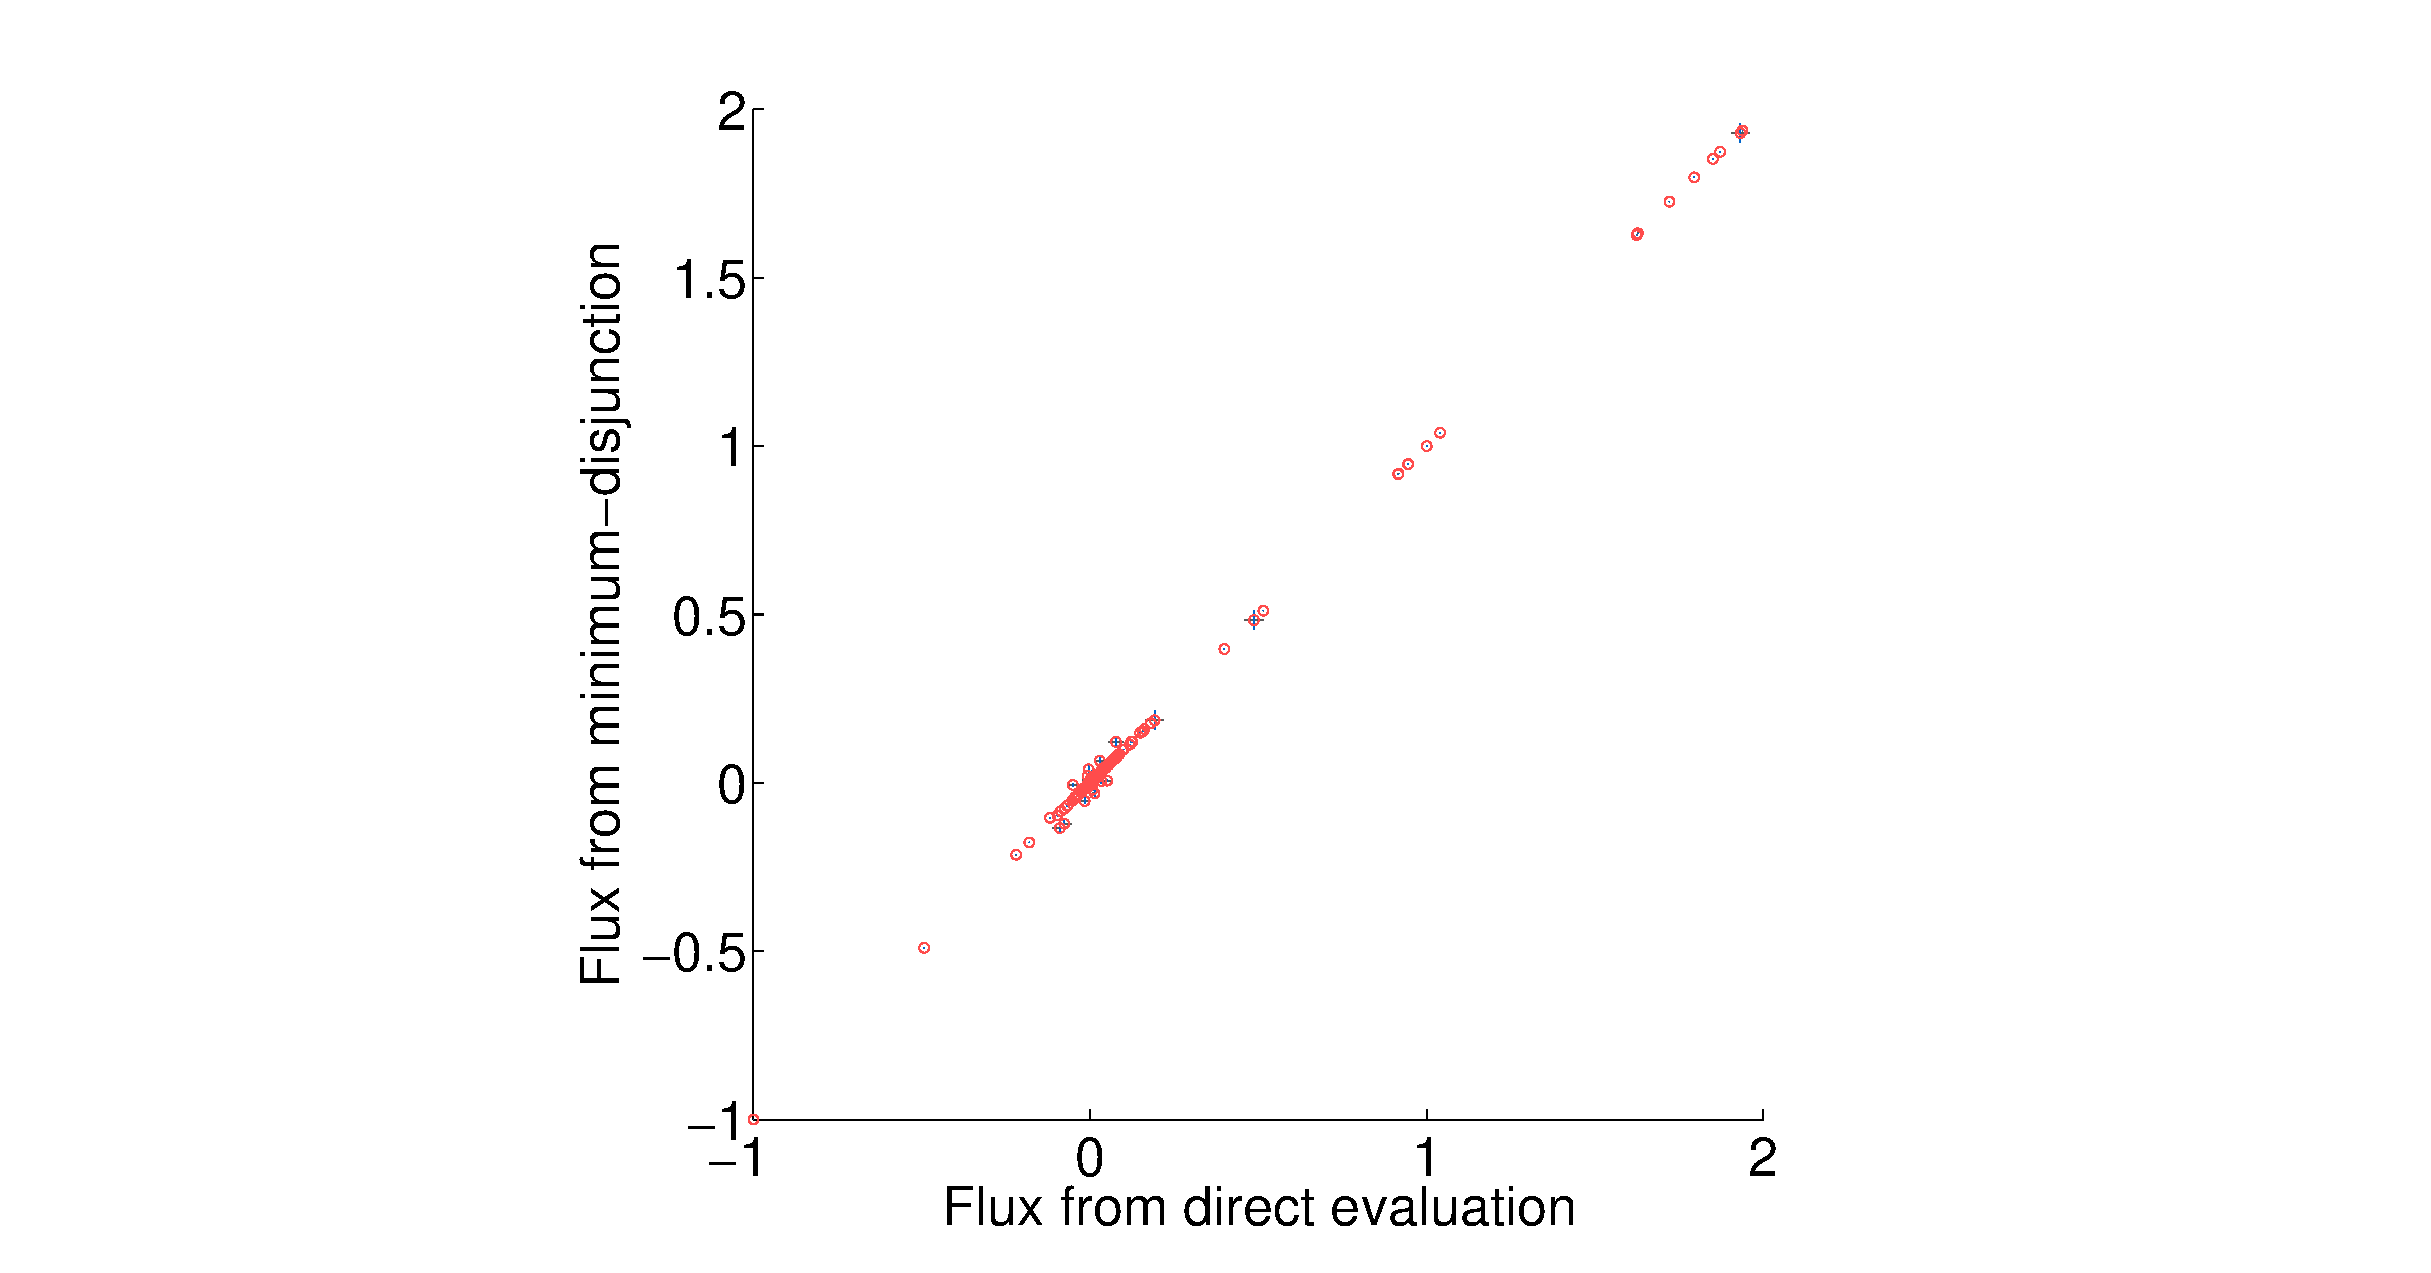
\includegraphics[width=\textwidth, trim=9cm 0cm 9cm 0cm, clip=true]
  {expCmpY7HC}
  \caption{highly constrained} \label{fig:EnzAbundEval:A}
  \end{subfigure}
&
  \begin{subfigure}[b]{0.5\textwidth}
  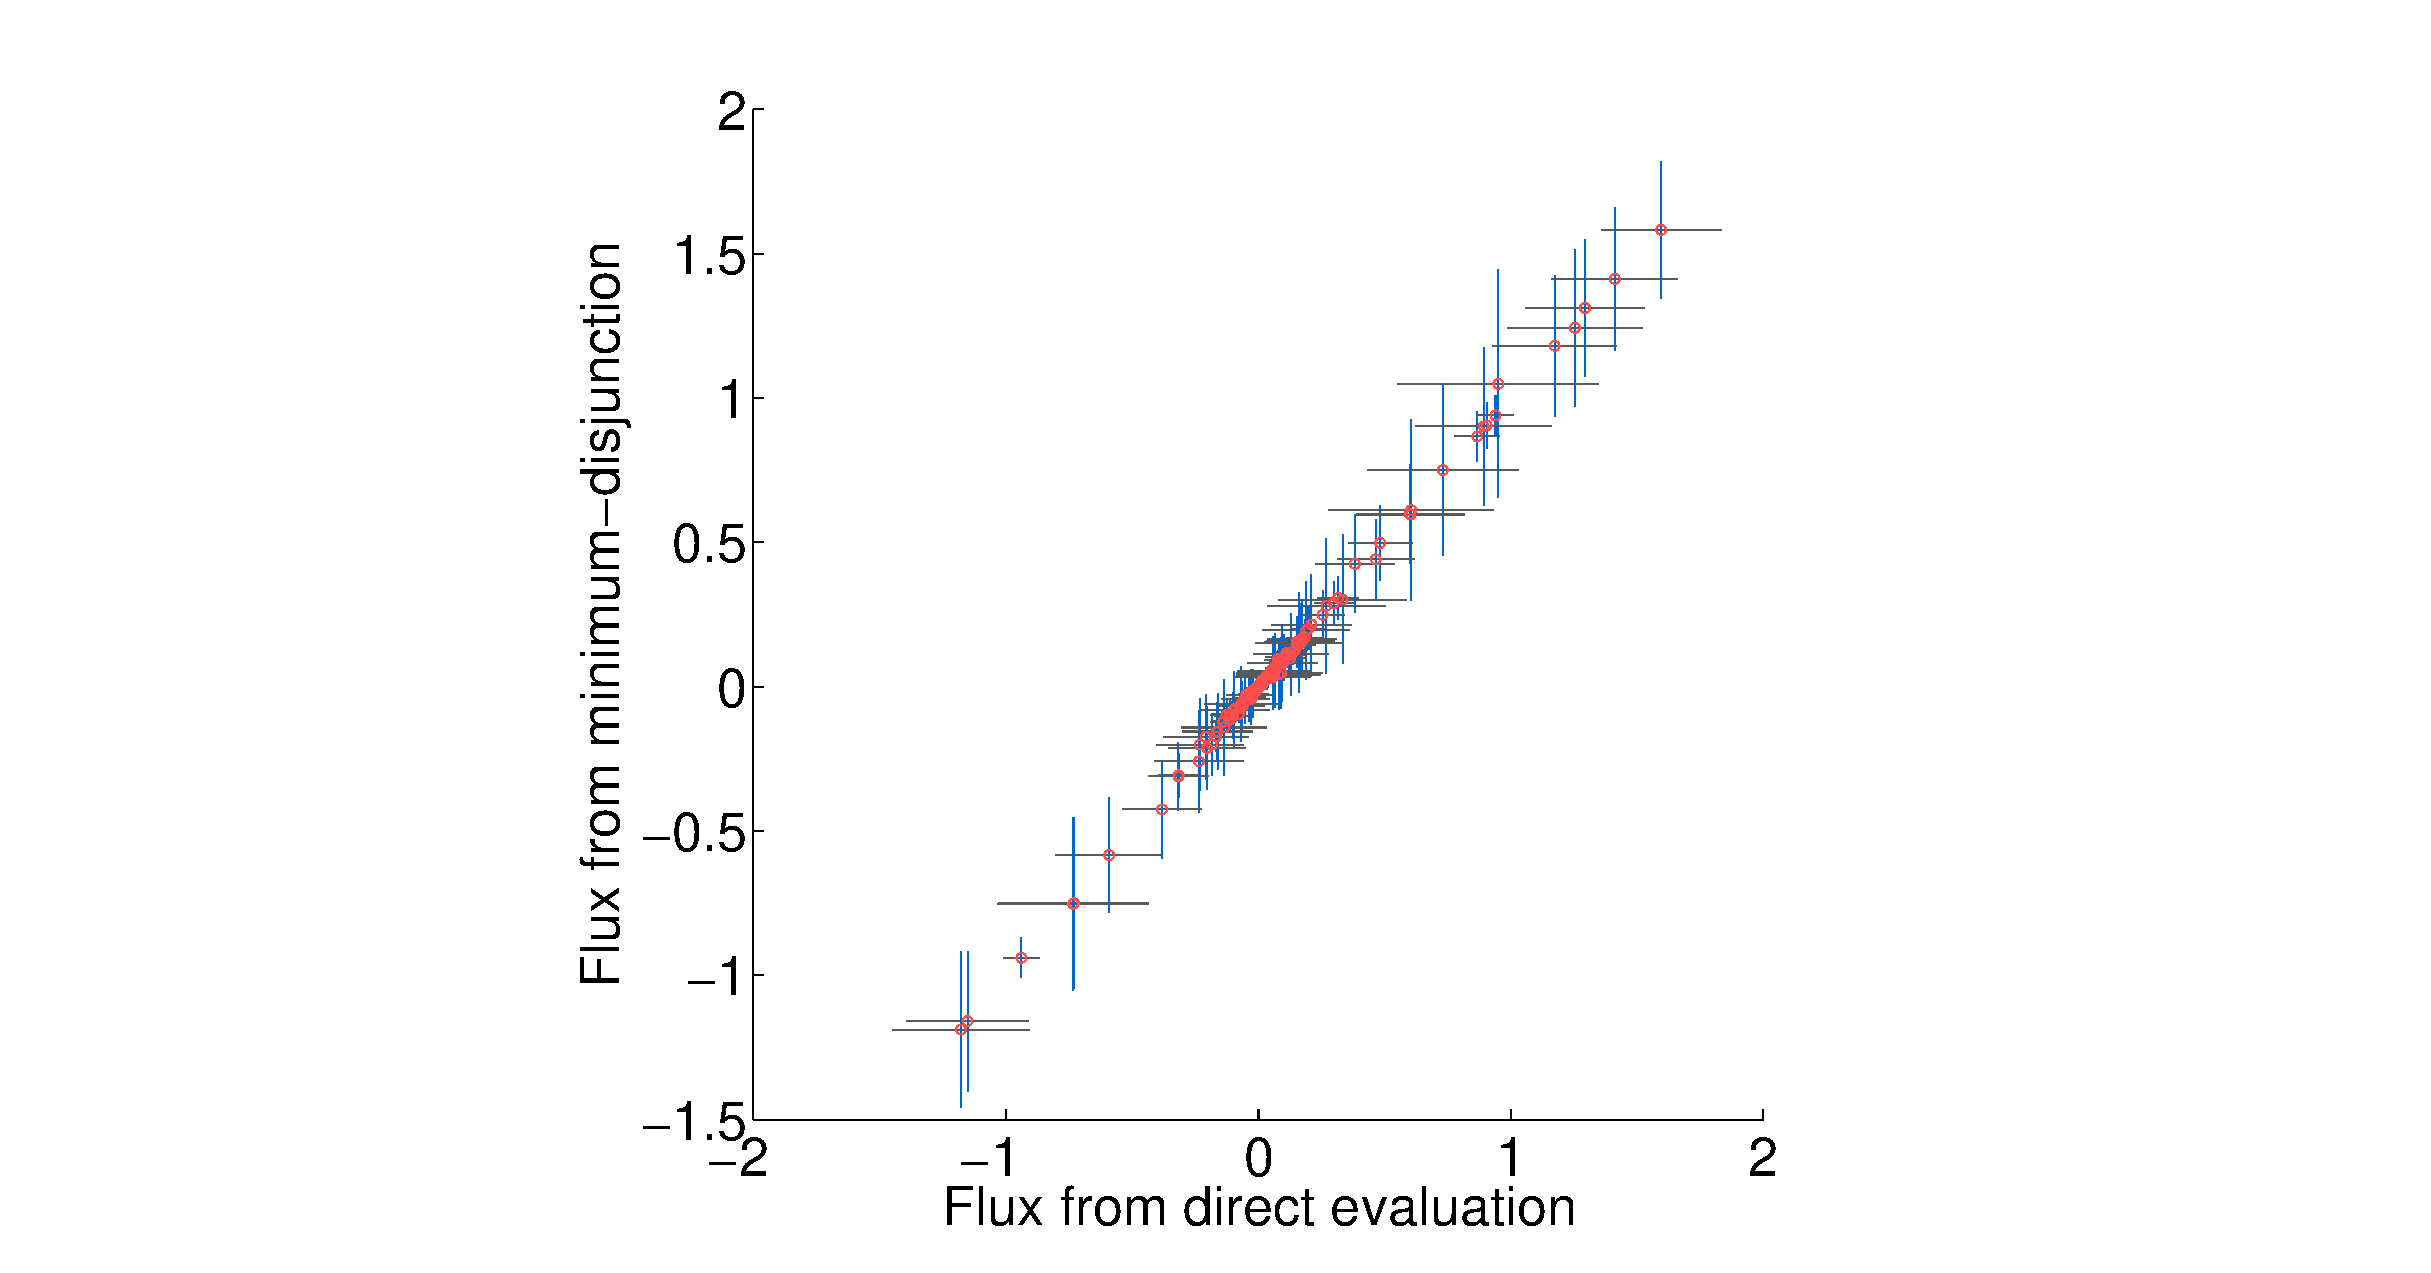
\includegraphics[width=\textwidth, trim=9cm 0cm 9cm 0cm, clip=true]
  {expCmpY7MC}
  \caption{minimally constrained} \label{fig:EnzAbundEval:B}
  \end{subfigure} 
\\
\end{tabular}
\vspace{-4mm}
\label{fig:EnzAbundEval}
\end{figure}
}


%%%%%%%%%%%%%%%%%%%%%%%%%%%%%%%%%%%%%%%%%%%%%%%%%%%%%%%%%%%%%%%%%%%%%%%%%%%%%%%%%%%%%%%%%%

\frame{\frametitle{Complexation effect in flux mapping: human} 

\begin{figure}
\centering
\begin{tabular}{cc}
  \begin{subfigure}[b]{0.5\textwidth}
  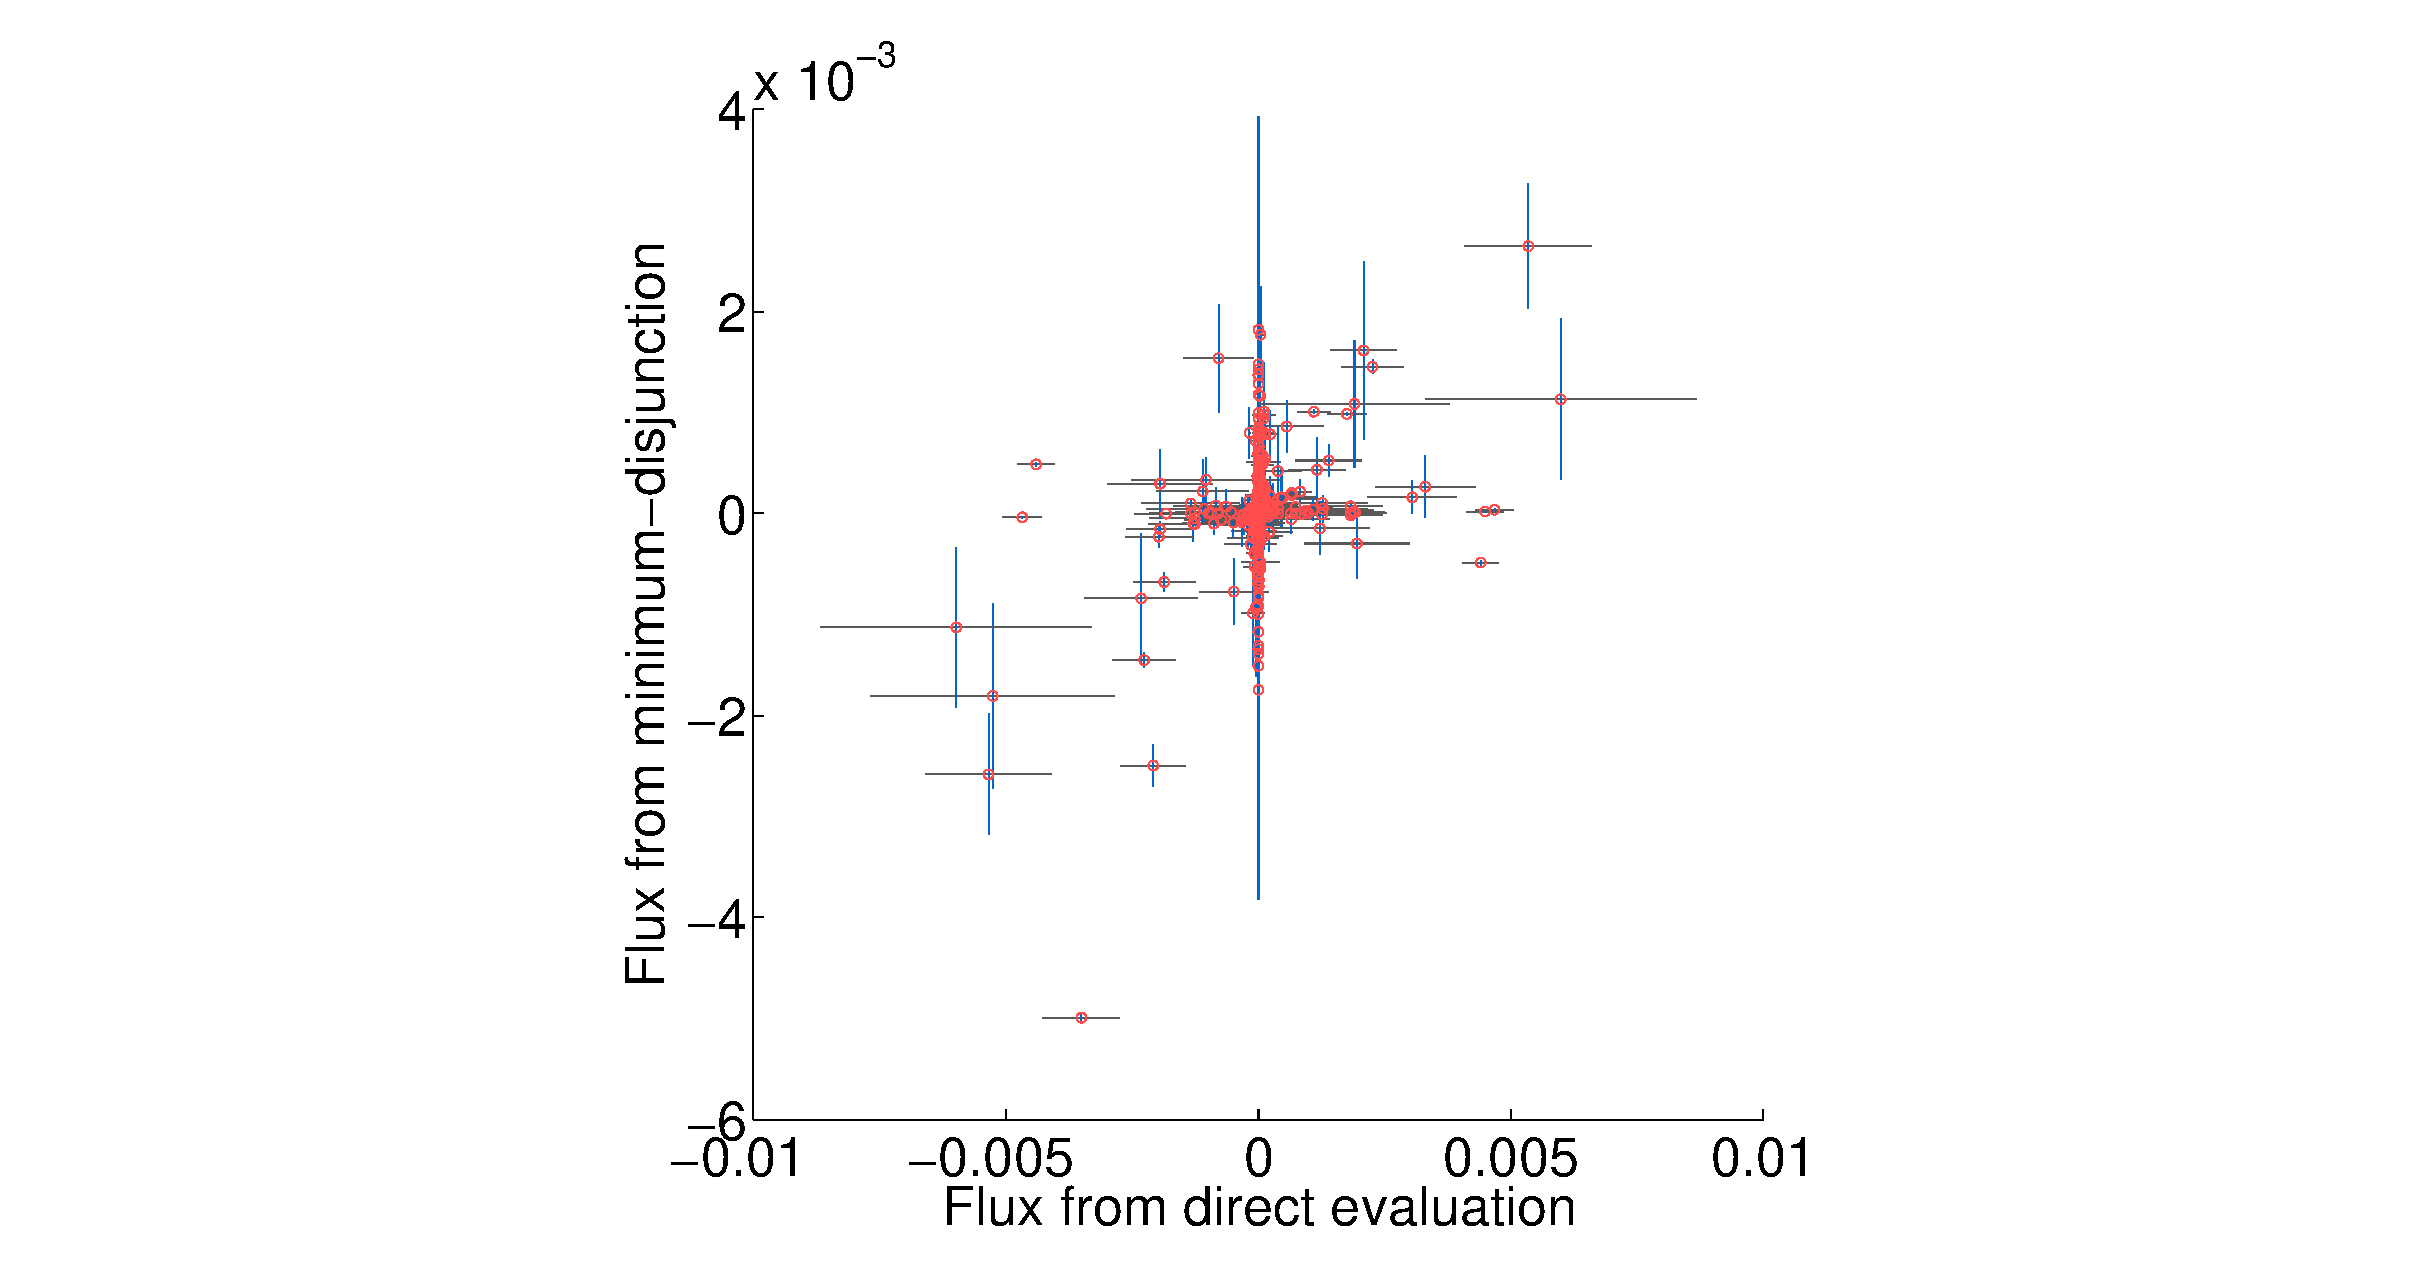
\includegraphics[width=\textwidth, trim=9cm 0cm 9cm 0cm, clip=true]
  {expCmpR2HC}
  \caption{highly constrained} \label{fig:EnzAbundEval:C}
  \end{subfigure}
&
  \begin{subfigure}[b]{0.5\textwidth}
  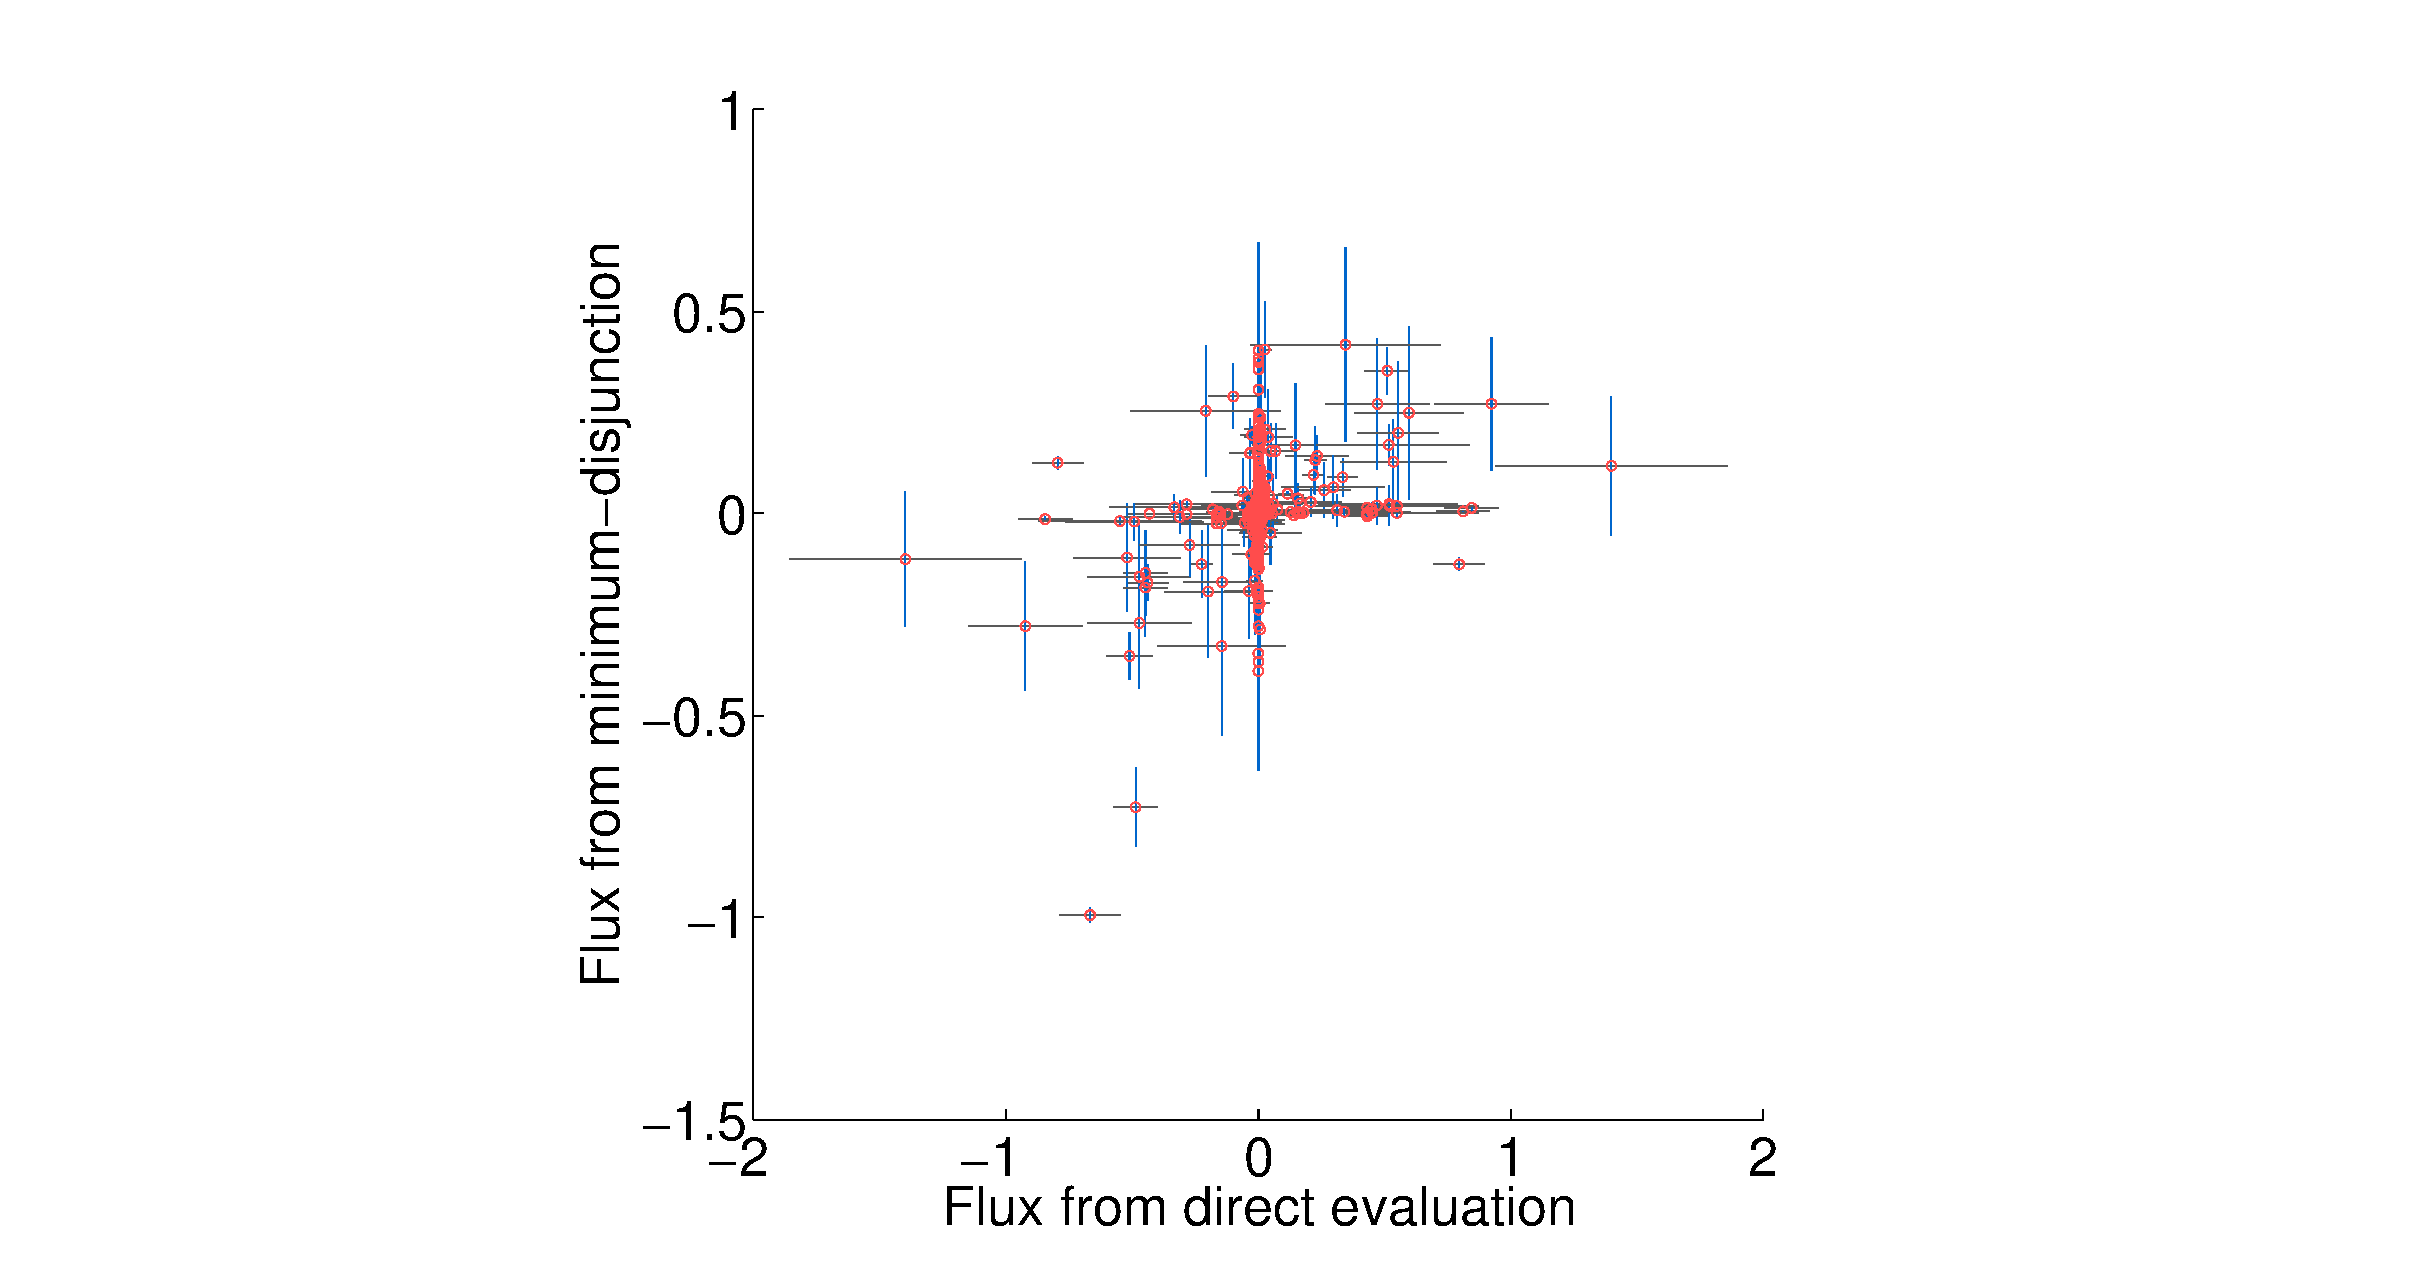
\includegraphics[width=\textwidth, trim=9cm 0cm 9cm 0cm, clip=true]
  {expCmpR2dC}
  \caption{minimally constrained} \label{fig:EnzAbundEval:D}
  \end{subfigure} 
\\
\end{tabular}
\vspace{-4mm}
\label{fig:EnzAbundEval}
\end{figure}
}

%%%%%%%%%%%%%%%%%%%%%%%%%%%%%%%%%%%%%%%%%%%%%%%%%%%%%%%%%%%%%%%%%%%%%%%%%%%%%%%%%%%%%%%%%%

%%%%%%%%%%%%%%%%%%%%
\section{Results}  %
%%%%%%%%%%%%%%%%%%%%

%%%%%%%%%%%%%%%%%%%%%%%%%%%%%%%%%%%%%%%%%%%%%%%%%%%%%%%%%%%%%%%%%%%%%%%%%%%%%%%%%%%%%%%%%%

\frame{\frametitle{Performance} 

\hl{break in to two slides}
\hl{highlight or do it as a bar graph}


\begin{figure}
\centering
\resizebox{\textwidth}{!}{%
\begin{tabular}{lrrrrrrrrr}
\textbf{(a)} \hspace{1.2cm} & Max. $\mu$ & Model & 
  Standard FBA & Fitted FBA & GIMME & iMAT & Lee et al. & FALCON\\
 & 75 \%& Yeast~5 MC & 0.66 & 0.66 & NaN  & 0.57 & 0.64 & 1 \\
 & 75 \%& Yeast~7 MC & 0.66 & 0.66 & 0.68 & 0.66 & 0.66 & 0.98\\
 & 75 \%& Yeast~5 HC & 0.73 & 0.78 & 0.75 & 0.66 & 0.98 & 0.99\\
Pearson's r  
 & 75 \%& Yeast~7 HC & 0.70 & 0.70 & 0.80 & 0.66 & 0.98 & 0.99\\
 & 85 \%& Yeast~7 MC & 0.62 & 0.62 & 0.65 & 0.62 & 0.62 & 0.97\\
 & 85 \%& Yeast~5 HC & 0.88 & 0.89 & 0.9  & 0.81 & 0.99 & 0.99\\
 & 85 \%& Yeast~7 HC & 0.67 & 0.67 & 0.87 & 0.62 & 0.98 & 0.98\\
\end{tabular}}
\resizebox{\textwidth}{!}{%
\begin{tabular}{lrrrrrrrrr}
\textbf{(b)} \hspace{1.2cm} & Max. $\mu$ & Model & 
  Standard FBA & Fitted FBA & GIMME & iMAT & Lee et al. & FALCON\\
 & 75 \%& Yeast~5 MC & 0.9  & 470   & 0.81  & 50     & 110 & 1.8 \\
 & 75 \%& Yeast~7 MC & 1.9  & 3,100 & 2.1   & 12,000 & 600 & 5.6 \\
 & 75 \%& Yeast~5 HC & 0.12 & 110   & 0.18  & 1.4    & 15  & 0.27\\
Time (s) 
 & 75 \%& Yeast~7 HC & 0.72 & 940   & 1.7   & 240    & 670 & 5.5 \\
 & 85 \%& Yeast~7 MC & 2.3  & 3,100 & 3.8   & 14,000 & 610 & 4.6 \\
 & 85 \%& Yeast~5 HC & 0.12 & 110   & 0.18  & 2.5    & 15  & 0.22\\
 & 85 \%& Yeast~7 HC & 0.70 & 110   & 2.5   & 100    & 530 & 5.9\\
\end{tabular}}
\caption{Performance of FALCON and other CBM methods for predicting
yeast exometabolic fluxes in two growth conditions (75~\% and 85~\%
Max.~$\mu$)}
\label{tab:FalcPerf}
\end{figure}
}

%%%%%%%%%%%%%%%%%%%%%%%%%%%%%%%%%%%%%%%%%%%%%%%%%%%%%%%%%%%%%%%%%%%%%%%%%%%%%%%%%%%%%%%%%%

\frame{\frametitle{Permuted expression validates fitting method} 
\hl{Show unbiasedness}

\begin{figure}
\centering
\begin{tabular}{cc}
  \begin{subfigure}[b]{0.5\textwidth}
  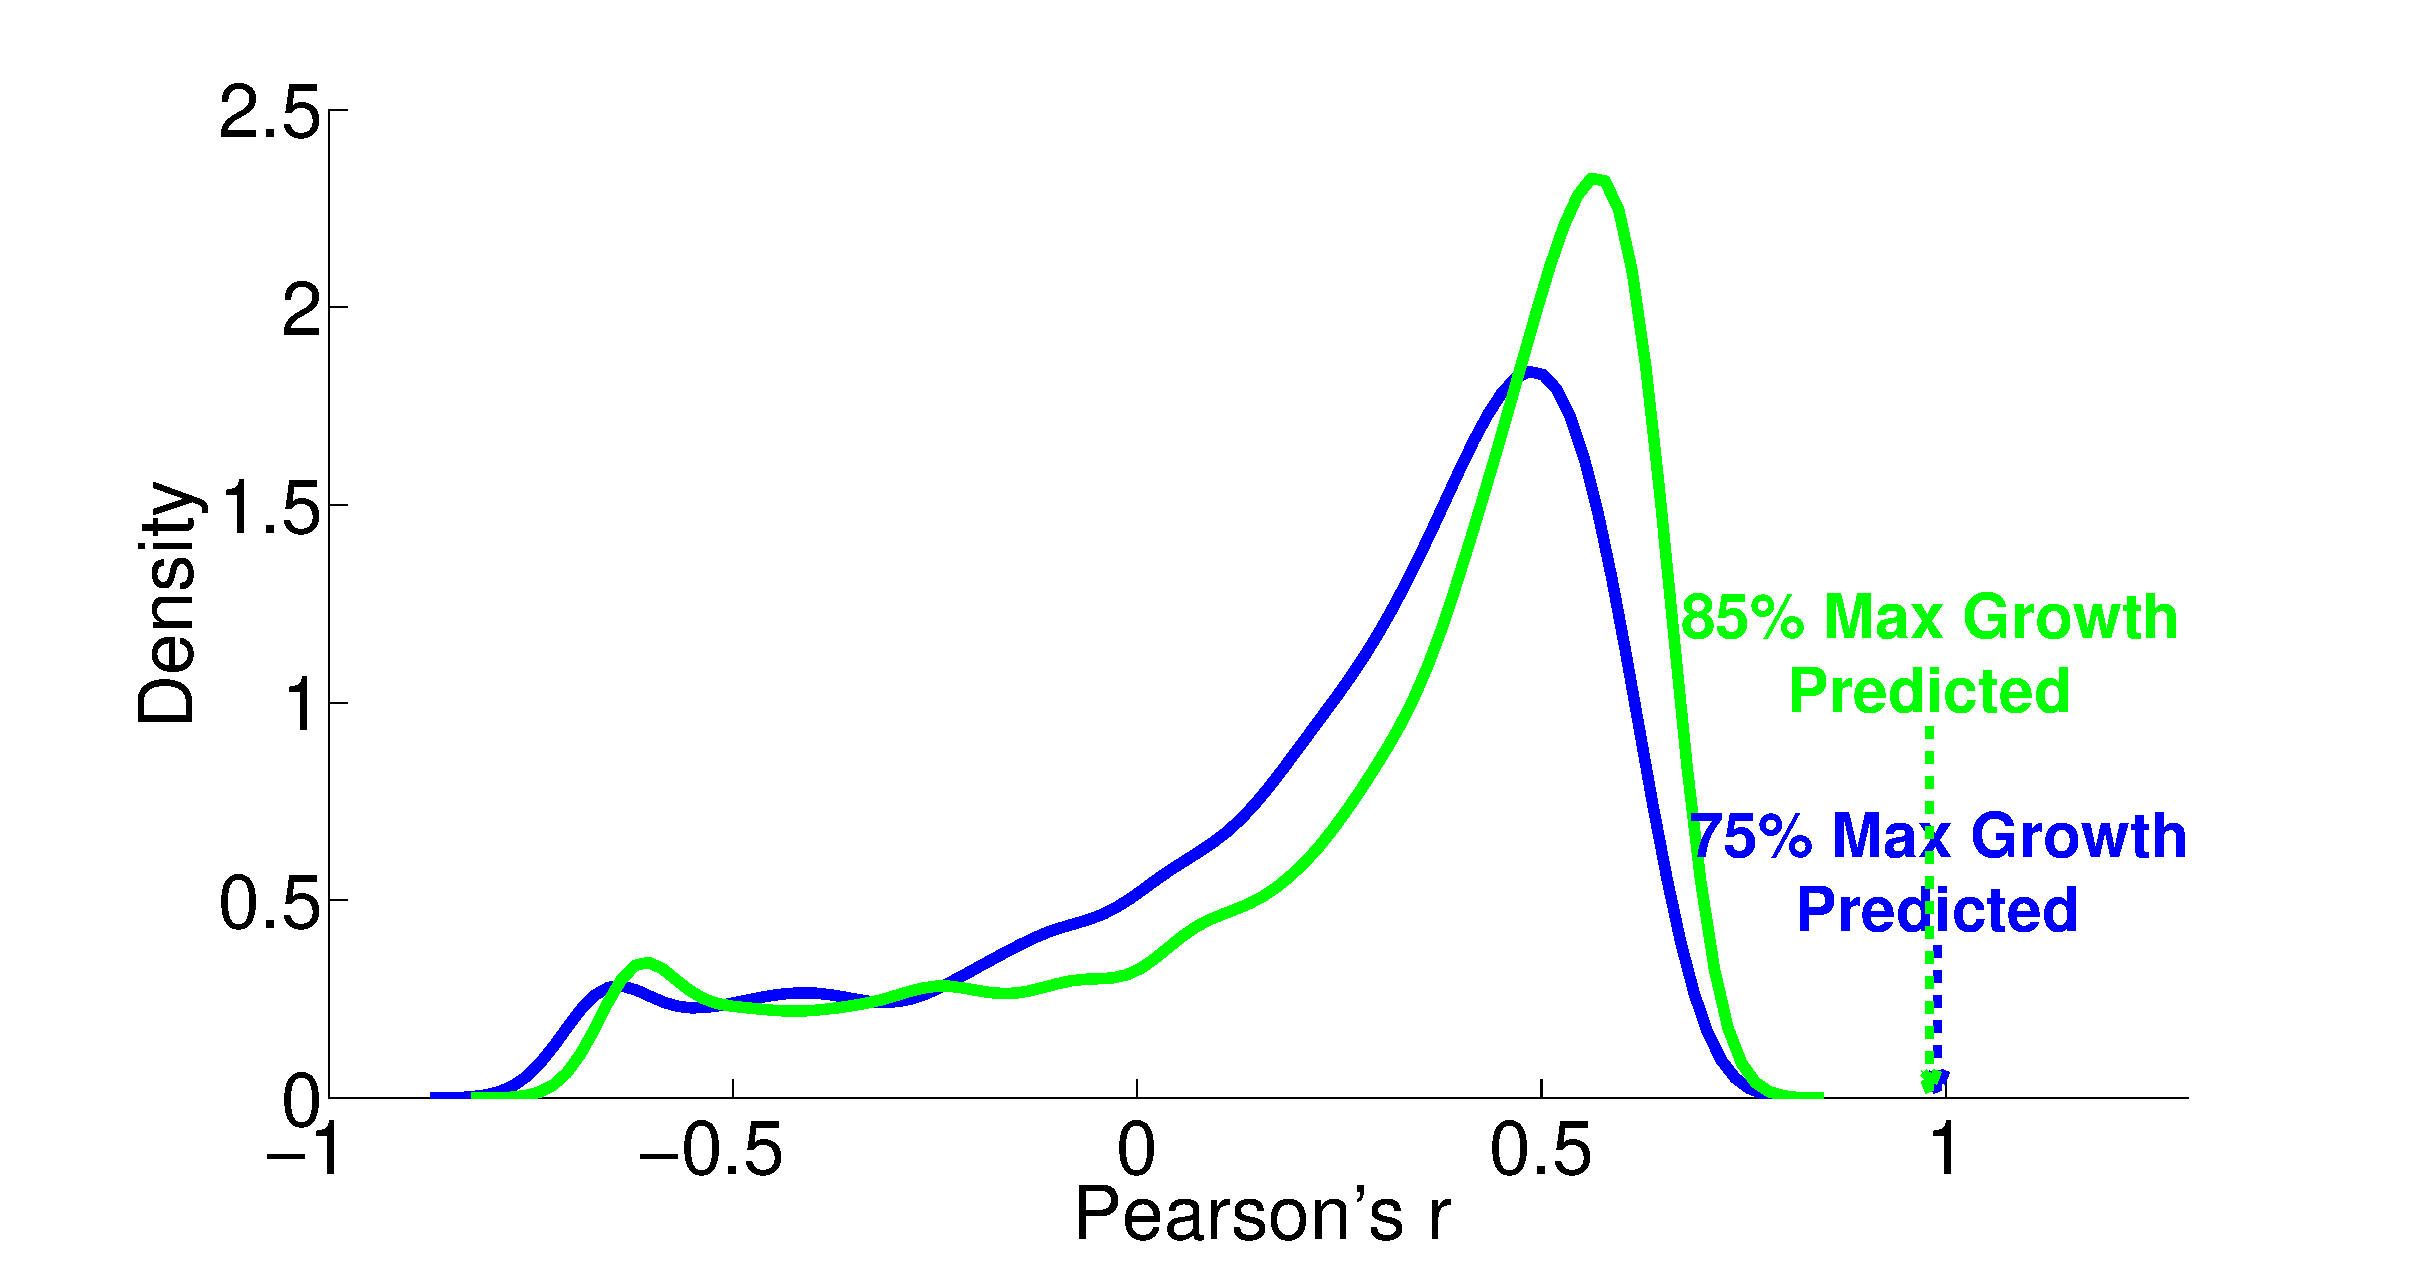
\includegraphics[width=\textwidth]{pExp}
  \caption{highly constrained} \label{fig:YpermCorr:A}
  \end{subfigure}
&
  \begin{subfigure}[b]{0.5\textwidth}
  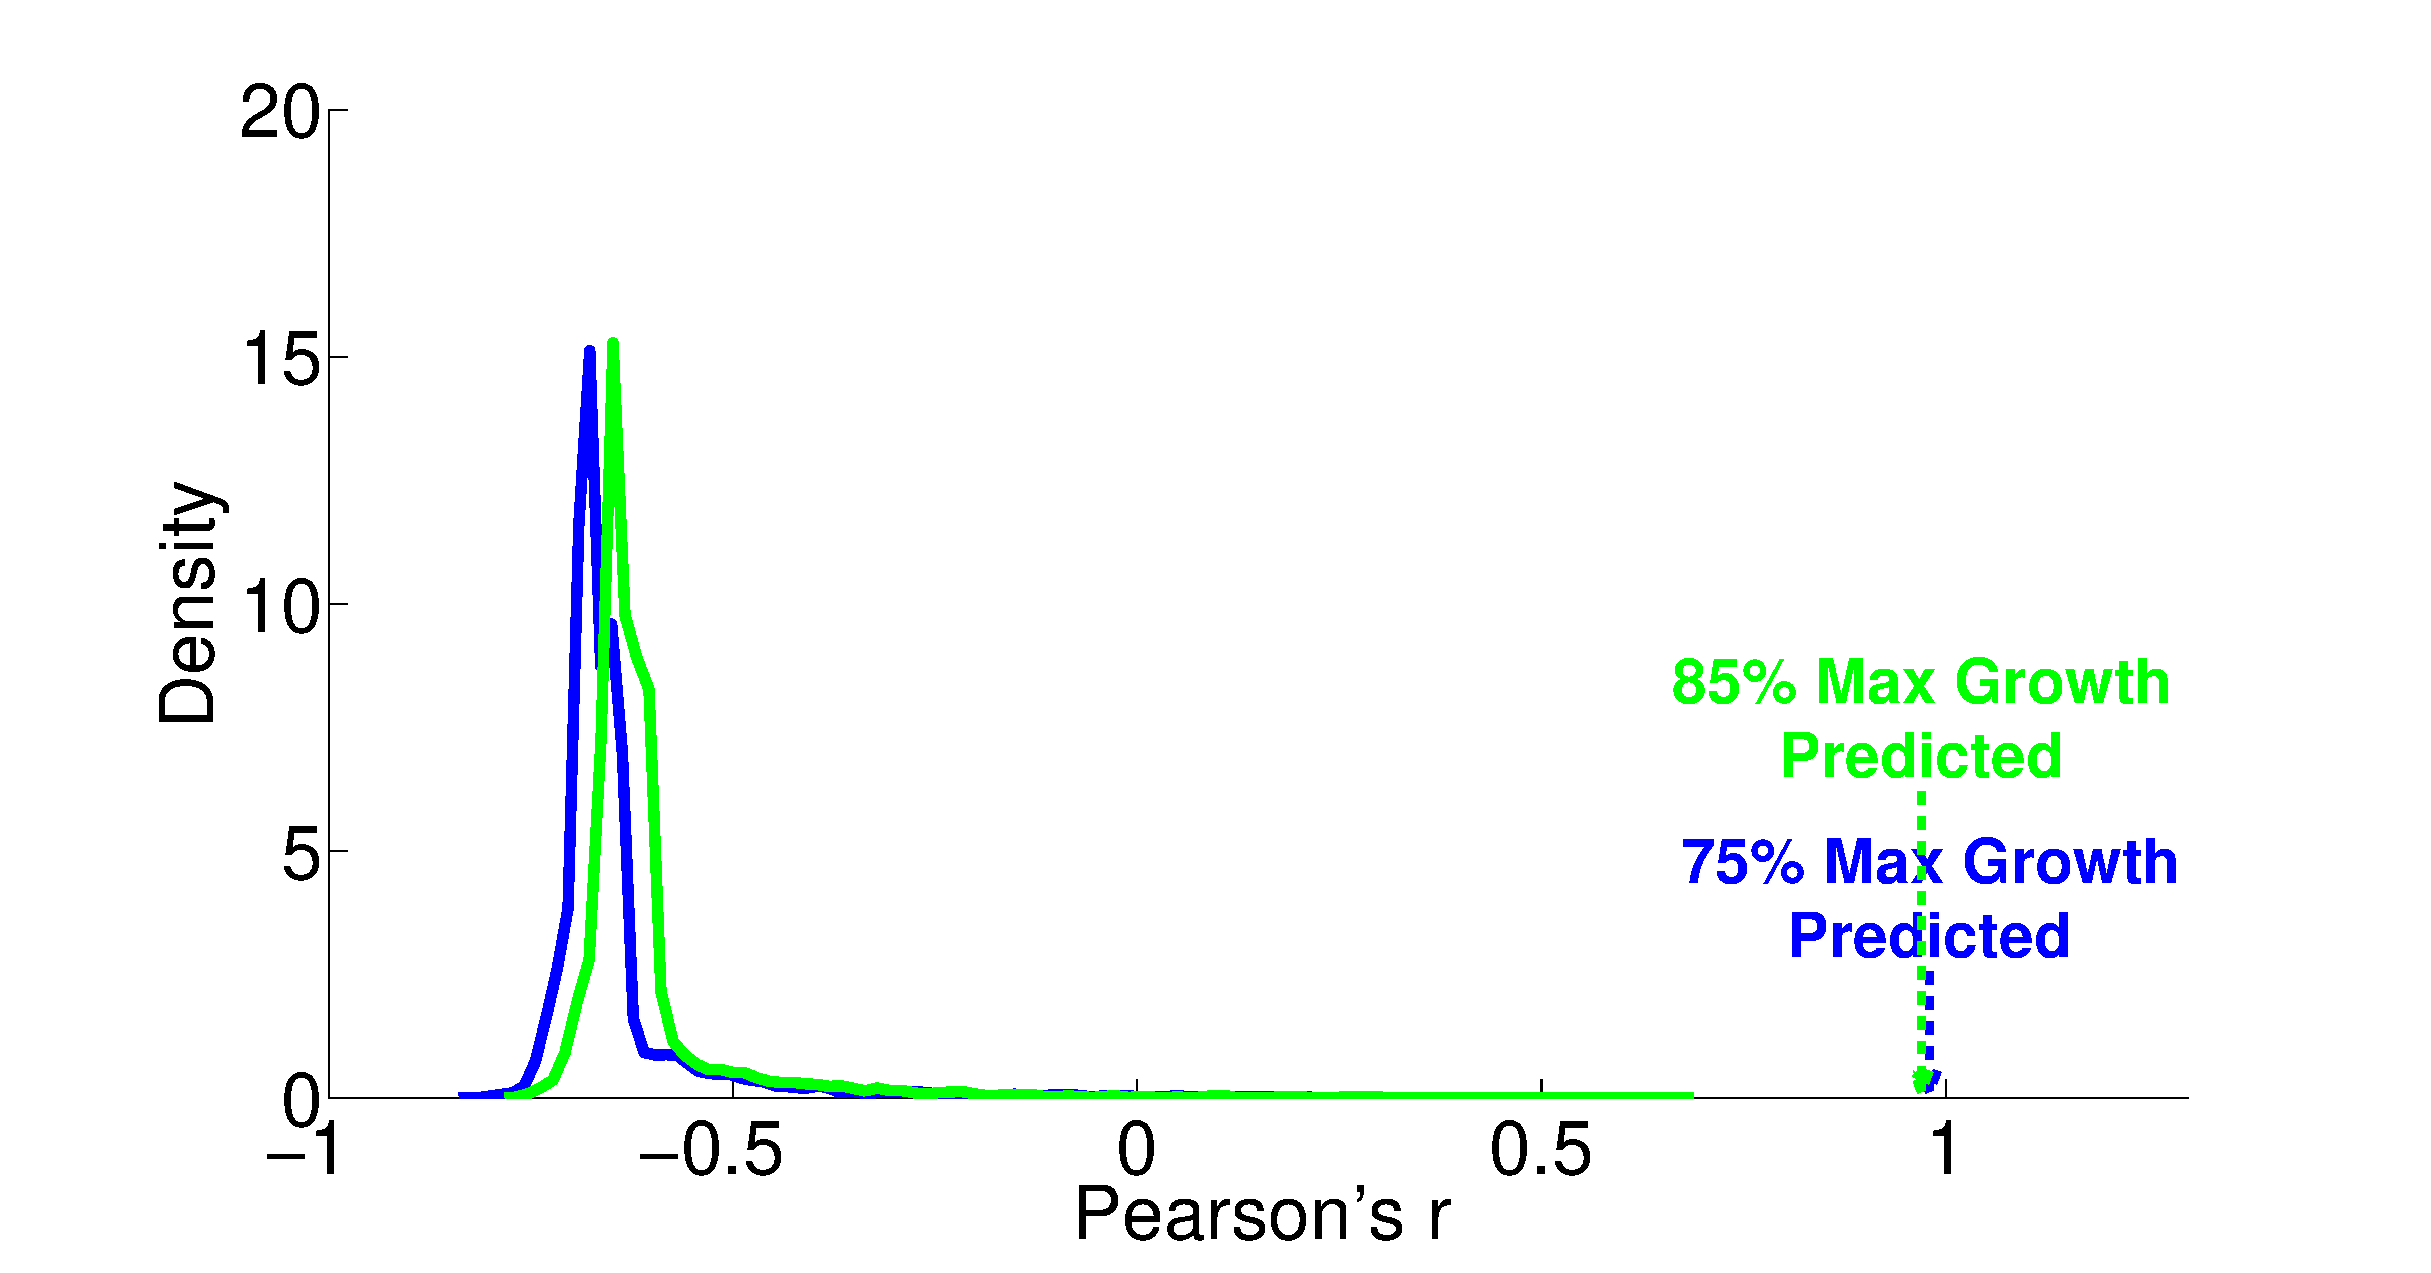
\includegraphics[width=\textwidth]{pExp_dirr}
  \caption{minimally constrained} \label{fig:YpermCorr:B}
  \end{subfigure} 
\\
\end{tabular}
\vspace{-4mm} 
\caption{PDFs of correlation between experimental fluxes and fluxes
estimated from FALCON when all gene expression data points are
permuted.}
\label{fig:YpermCorr}
\end{figure}
}

%%%%%%%%%%%%%%%%%%%%%%%%%%%%%%%%%%%%%%%%%%%%%%%%%%%%%%%%%%%%%%%%%%%%%%%%%%%%%%%%%%%%%%%%%%


%%%%%%%%%%%%%%%%%%%%%%%%%%%%%%%%%%%%%%%%%%%%%%%%%%%%%%%%%%%%%%%%%%%%%%%%%%%%%%%%%%%%%%%%%%

\frame{\frametitle{Correlation of perturbed inputs (complex abundance)} 
\hl{only show one in main text}

\begin{figure}
\centering
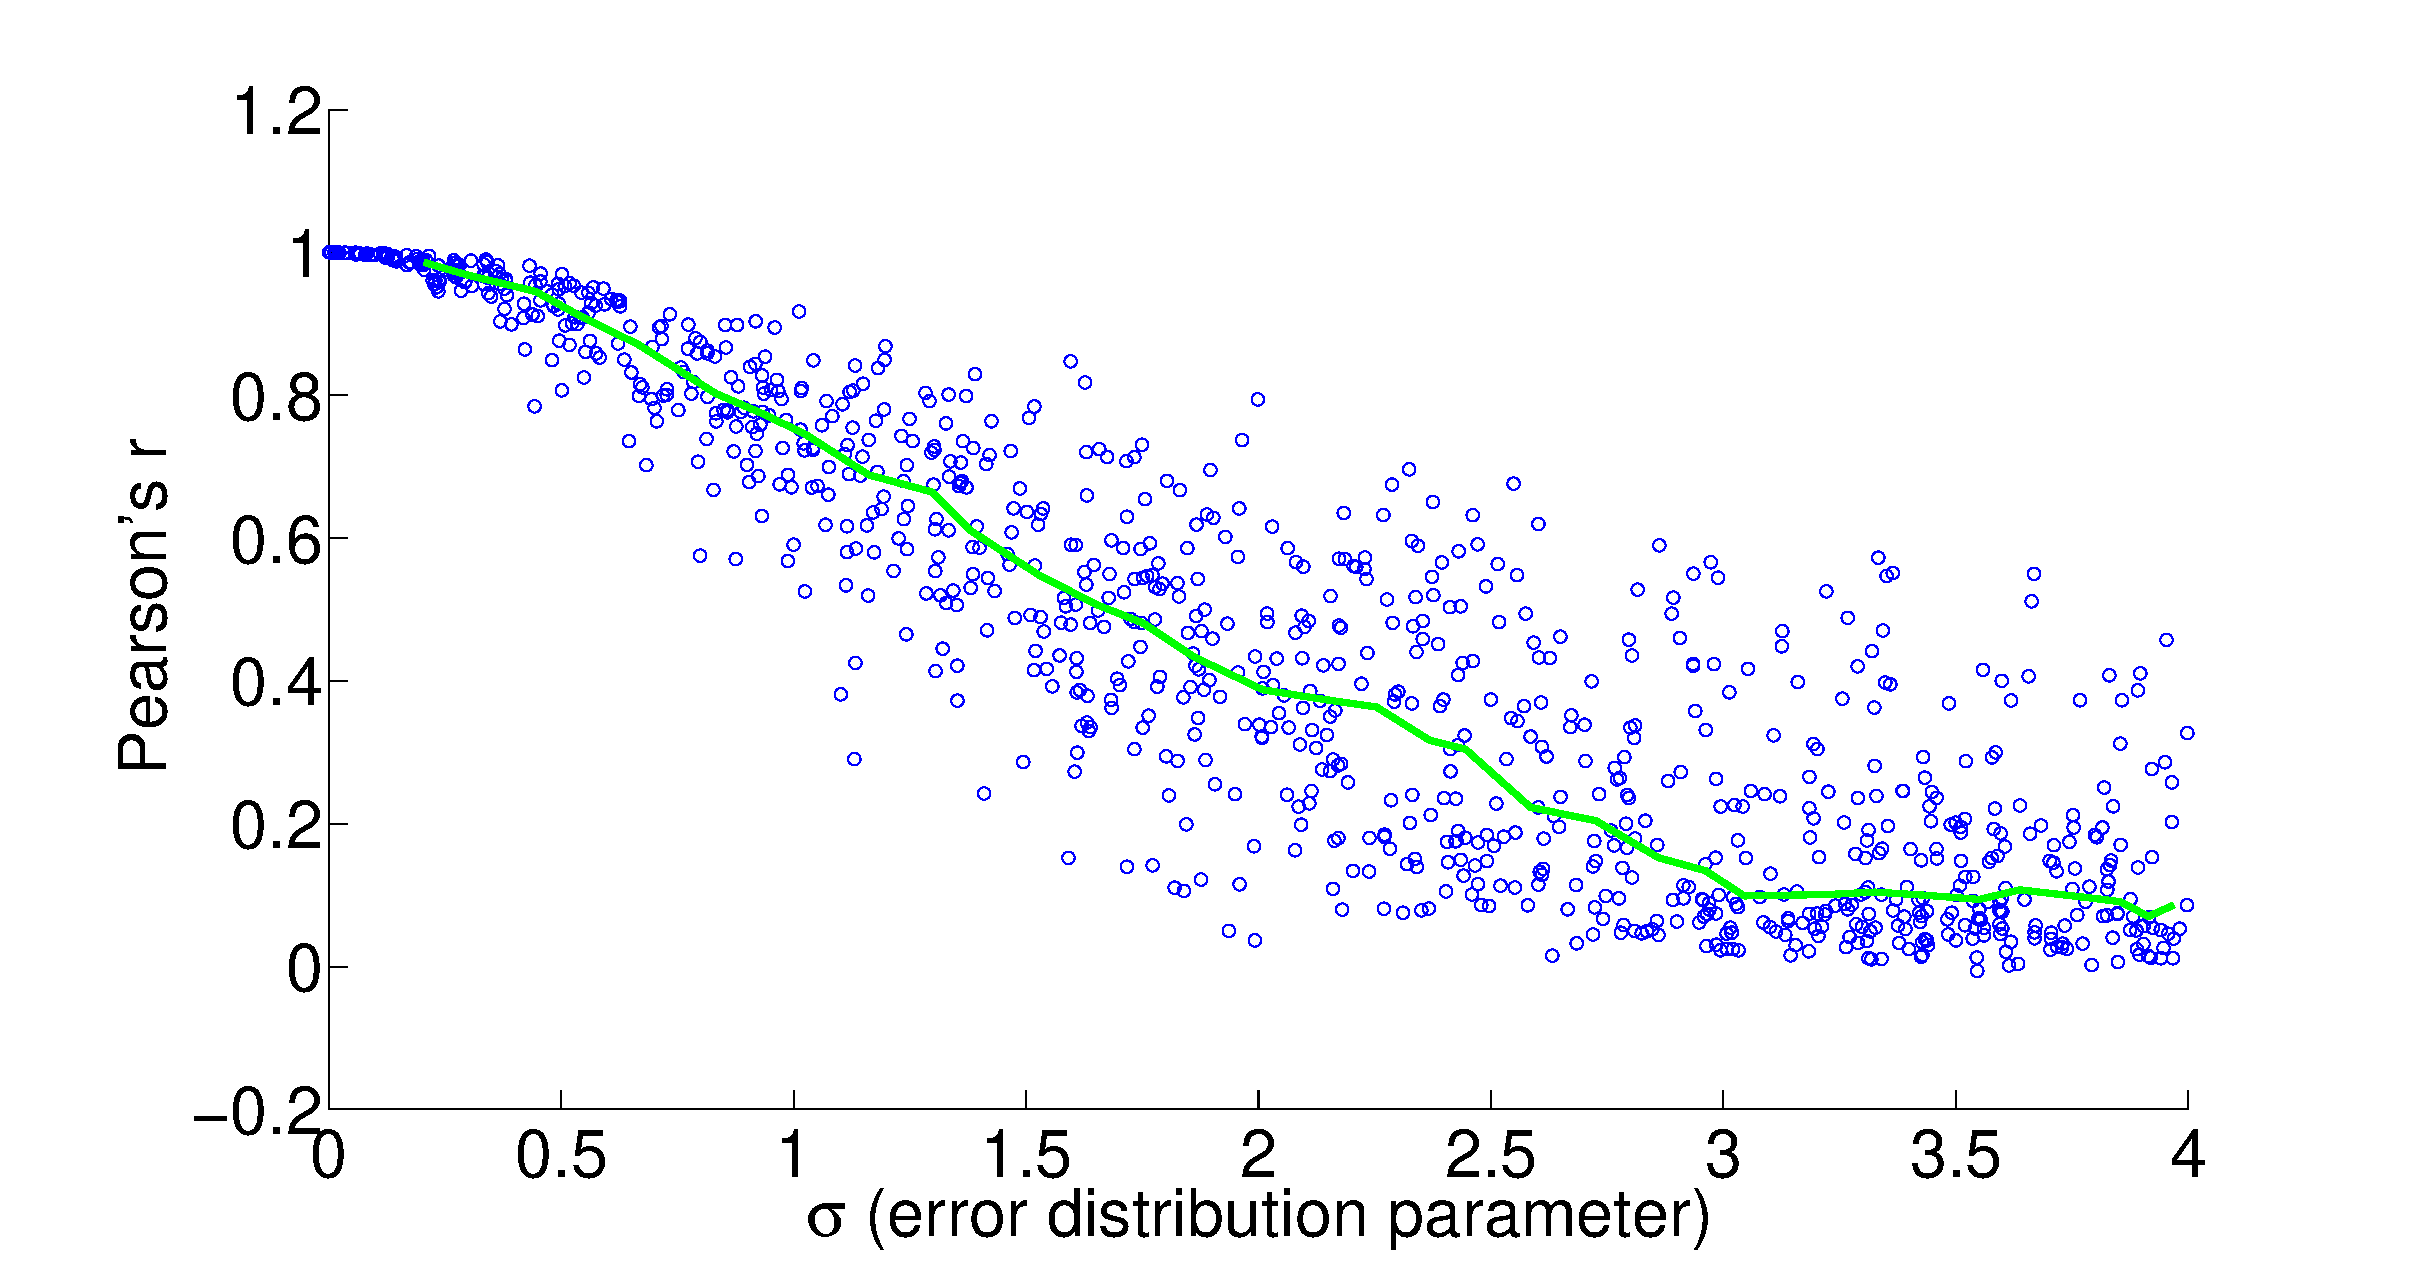
\includegraphics[width=\textwidth]{noise_y7EC}
\caption{Correlation of perturbed enzyme abundance vectors with the
associated unperturbed vector for the Yeast~7 model.}
\label{fig:ExpSens:Complex}
\end{figure}

}

%%%%%%%%%%%%%%%%%%%%%%%%%%%%%%%%%%%%%%%%%%%%%%%%%%%%%%%%%%%%%%%%%%%%%%%%%%%%%%%%%%%%%%%%%%

\frame{\frametitle{Sensitivity to expression noise} 

\begin{figure}
\centering
\begin{tabular}{cc}
  \begin{subfigure}[b]{0.5\textwidth}
  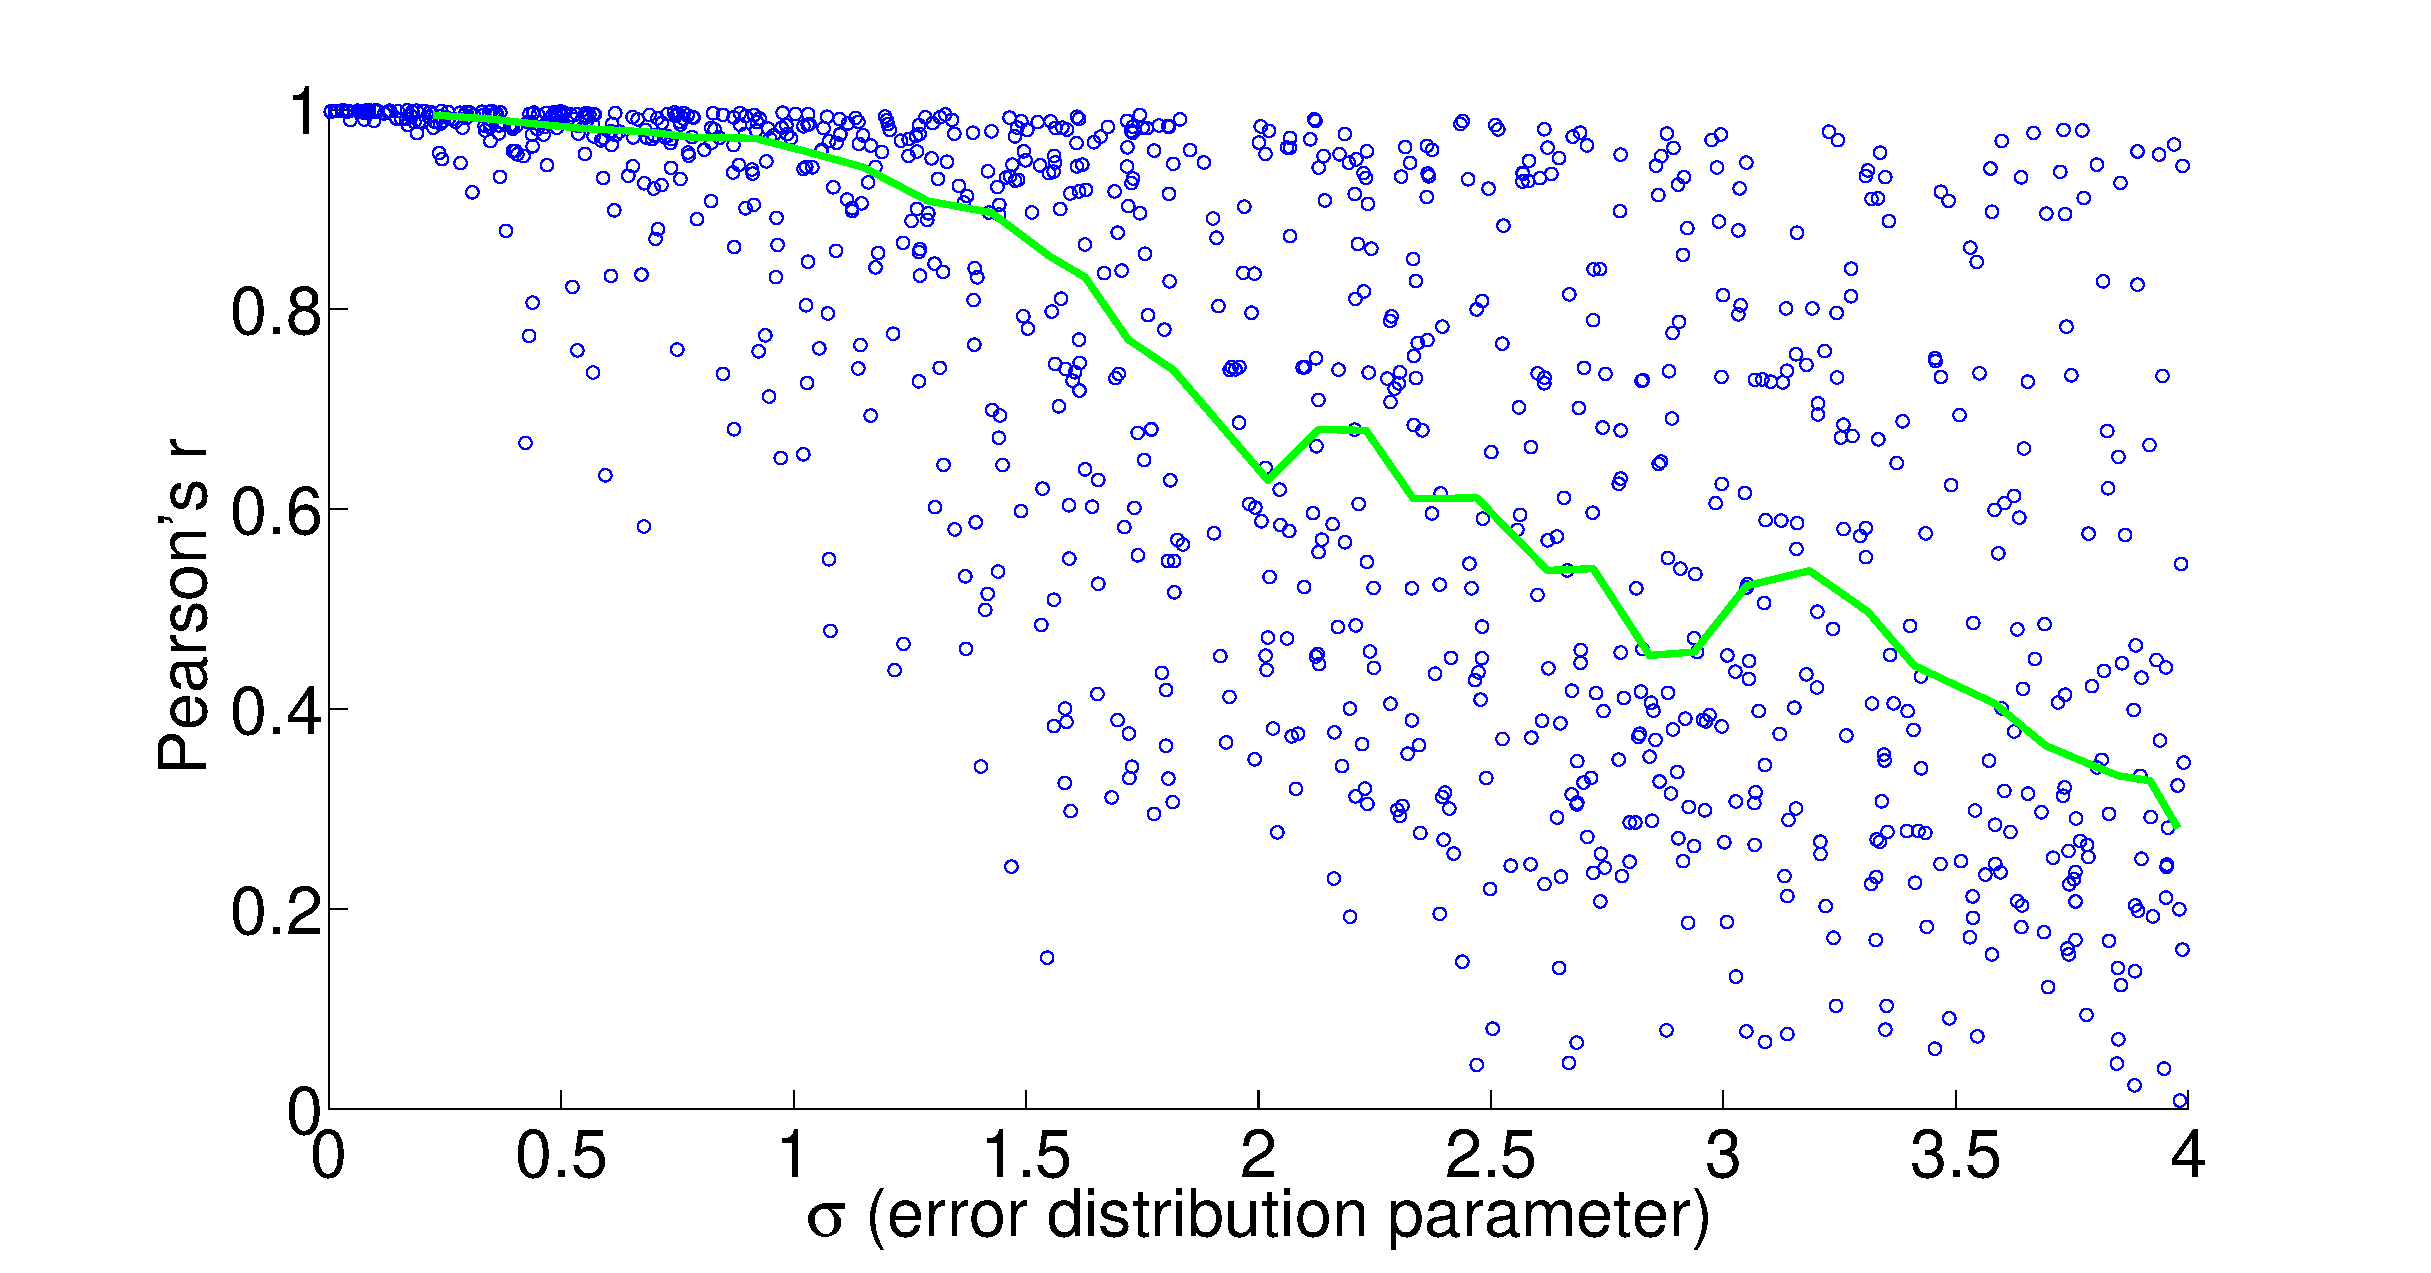
\includegraphics[width=\textwidth]{noise_y7HCflux}
  \caption{flux: highly constrained} \label{fig:ExpSens:B}
  \end{subfigure} 
&
  \begin{subfigure}[b]{0.5\textwidth}
  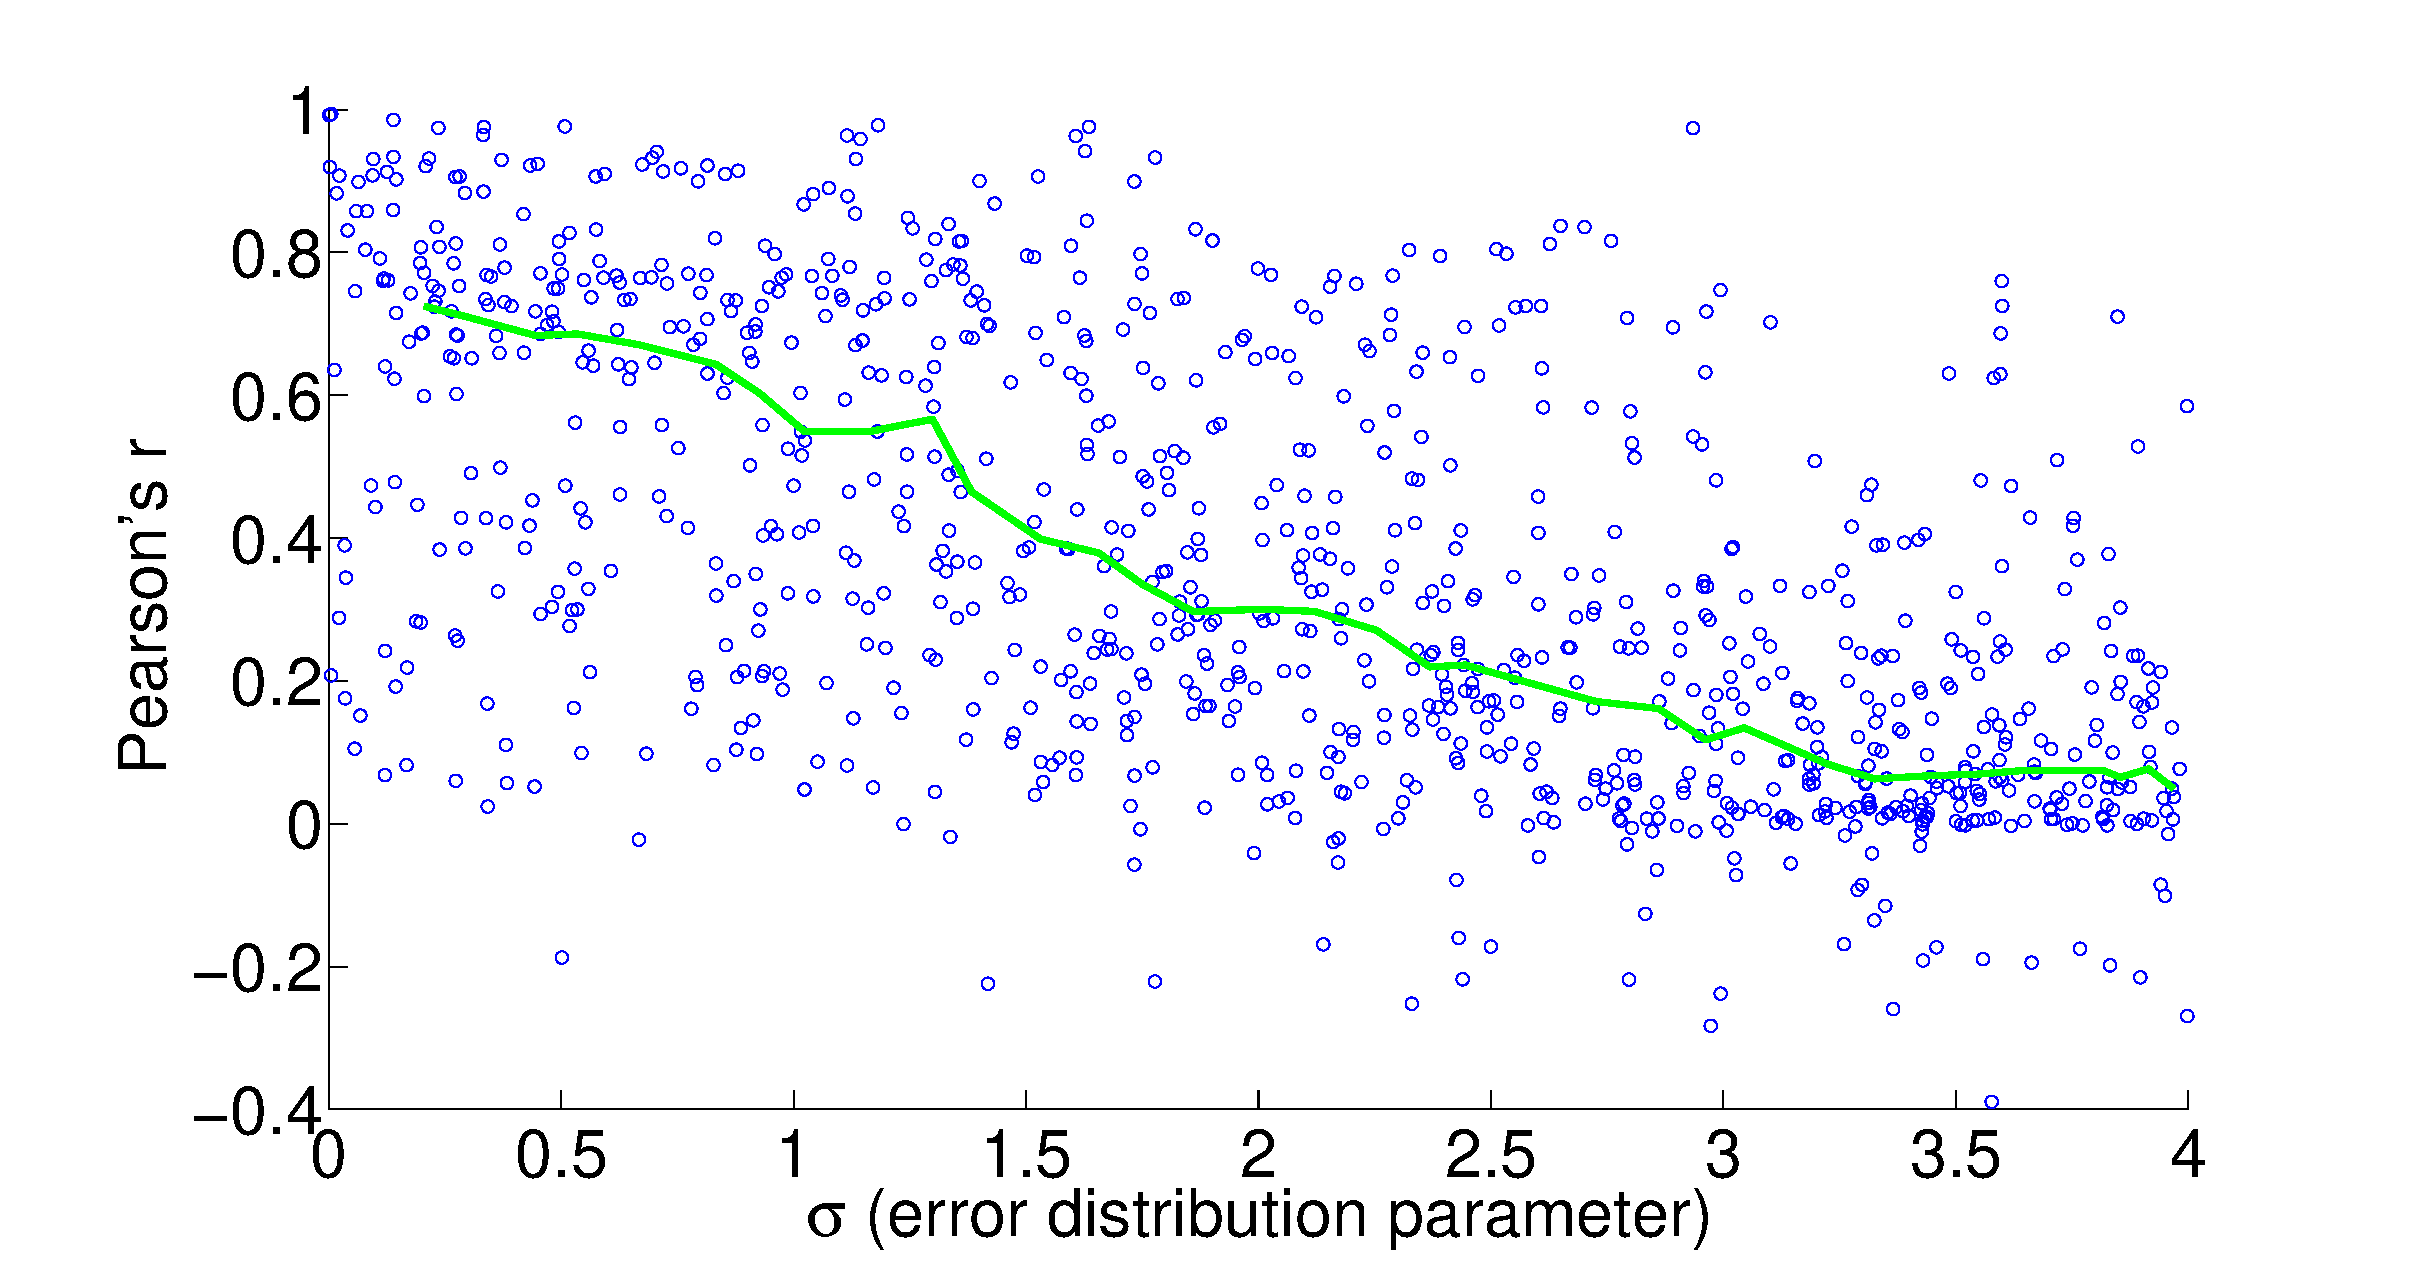
\includegraphics[width=\textwidth]{noise_y7MCflux}
  \caption{flux: minimally constrained} \label{fig:ExpSens:C}
  \end{subfigure} 
\\
\end{tabular}
\vspace{-4mm} 
\caption{Correlation of flux vectors estimated from perturbed versus
unperturbed complex abundance for the Yeast~7 model.}
\label{fig:ExpSens}
\end{figure}
}

%%%%%%%%%%%%%%%%%%%%%%%%%%%%%%%%%%%%%%%%%%%%%%%%%%%%%%%%%%%%%%%%%%%%%%%%%%%%%%%%%%%%%%%%%%

%%%%%%%%%%%%%%%%%%%%%%
                     %
\section{Discussion} %
                     %
%%%%%%%%%%%%%%%%%%%%%%

%%%%%%%%%%%%%%%%%%%%%%%%%%%%%%%%%%%%%%%%%%%%%%%%%%%%%%%%%%%%%%%%%%%%%%%%%%%%%%%%%%%%%%%%%%

%%%%%%%%%%%%%%%%%%%%%%%%%%%%%%%%%%%%%%%%%%%%%%%%%%%%%%%%%%%%%%%%%%%%%%%%%%%%%%%%%%%%%%%%%%

%%%%%%%%%%%%%%%%%%%%%%%%%%%%%
                            %
\section{Future Directions} %
                            %
%%%%%%%%%%%%%%%%%%%%%%%%%%%%%

%%%%%%%%%%%%%%%%%%%%%%%%%%%%%%%%%%%%%%%%%%%%%%%%%%%%%%%%%%%%%%%%%%%%%%%%%%%%%%%%%%%%%%%%%%

\frame{
\frametitle{Large-scale coupled simulations will be important} 

\begin{columns}[onlytextwidth]
%
\begin{column}{0.4\textwidth}

\begin{itemize}
  \footnotesize
  \item Expression is available for nearly all cell types.
  \item Can simulate tissues, microbial ecosystems, and multicellular organisms.
  \item Amenable to distributed computing.
  \begin{itemize}
    \scriptsize
    \item Cells only need to talk to neighboring cells.
    \item Only a small vector of concentration data needs needs to be passed.
  \end{itemize}
\end{itemize}
\end{column}
%
\begin{column}{0.6\textwidth}
\begin{figure}
\hfill\begin{flushleft}
\ul{Millions of pairwise simulations reveal\\ trends and complex genetic interactions.}
\end{flushleft}
\centering
\includegraphics[width=\textwidth]{Figure_S2}
\caption{\textit{Xu, Barker and Gu. PNAS, 2012.}}
\end{figure}
\end{column}
%
\end{columns}  
}

%%%%%%%%%%%%%%%%%%%%%%%%%%%%%%%%%%%%%%%%%%%%%%%%%%%%%%%%%%%%%%%%%%%%%%%%%%%%%%%%%%%%%%%%%%

\frame{\frametitle{Thank you!} 

TODO:\\
% Maybe use \only http://stackoverflow.com/questions/4683093/beamer-how-to-show-images-as-step-by-step-images
Remove highly and minimally constrained from slides.\\
Think more about title - catch the audience.\\
Add one slide talking about systems management in past\\
% Talk about metabolism, but not gene expression here.
% Applications to disease?
---also talk about parallel programming slide.\\
Add intro slide for context of metabolism.\\
Maybe add a table of function calls\\
Finish Thanks slide.\\
List new improvements to flux fitting.\\
Step through code blocks.\\
Correction section advancement at top of slide.\\
Spellcheck!\\

% \begin{columns}
% %
% \begin{column}
% Testing 
% % \begin{itemize}
% % \item Zhenglong Gu
% % \item Jason W. Locasale
% % \item Christopher R. Myers
% % \item Narayanan Sadagopan
% % \item Kieran Smallbone
% % \item Yiping Wang
% % \item Hongwei Xi
% \end{itemize}

% \end{column}
% \end{columns}

% % \begin{itemize}
% % \item David Christini 
% % \item Michael Stillman
% % \item Neil Swainston
% % \item Lin Xu
% % \item Tri-I CBM
% % \item Cornell's CAC
% % \end{itemize}
% % \end{column}
% % %
% % \begin{column}
% % Testing
% % \end{column}
% % %
% % \end{columns}
}

%%%%%%%%%%%%%%%%%%%%%%%%%%%%%%%%%%%%%%%%%%%%%%%%%%%%%%%%%%%%%%%%%%%%%%%%%%%%%%%%%%%%%%%%%%

%%%%%%%%%%%%%%%%%%%%%%%%%%%%%%%%
                               %
\section[]{Additional Slides}  %
                               %
%%%%%%%%%%%%%%%%%%%%%%%%%%%%%%%%

%%%%%%%%%%%%%%%%%%%%%%%%%%%%%%%%%%%%%%%%%%%%%%%%%%%%%%%%%%%%%%%%%%%%%%%%%%%%%%%%%%%%%%%%%%

\frame{\frametitle{}} %blank slide

%%%%%%%%%%%%%%%%%%%%%%%%%%%%%%%%%%%%%%%%%%%%%%%%%%%%%%%%%%%%%%%%%%%%%%%%%%%%%%%%%%%%%%%%%%

\frame{\frametitle{Global flux correlations from permuted inputs} 

\begin{figure}[!htb]
\centering
\begin{tabular}{cc}
  \begin{subfigure}[b]{0.5\textwidth}
  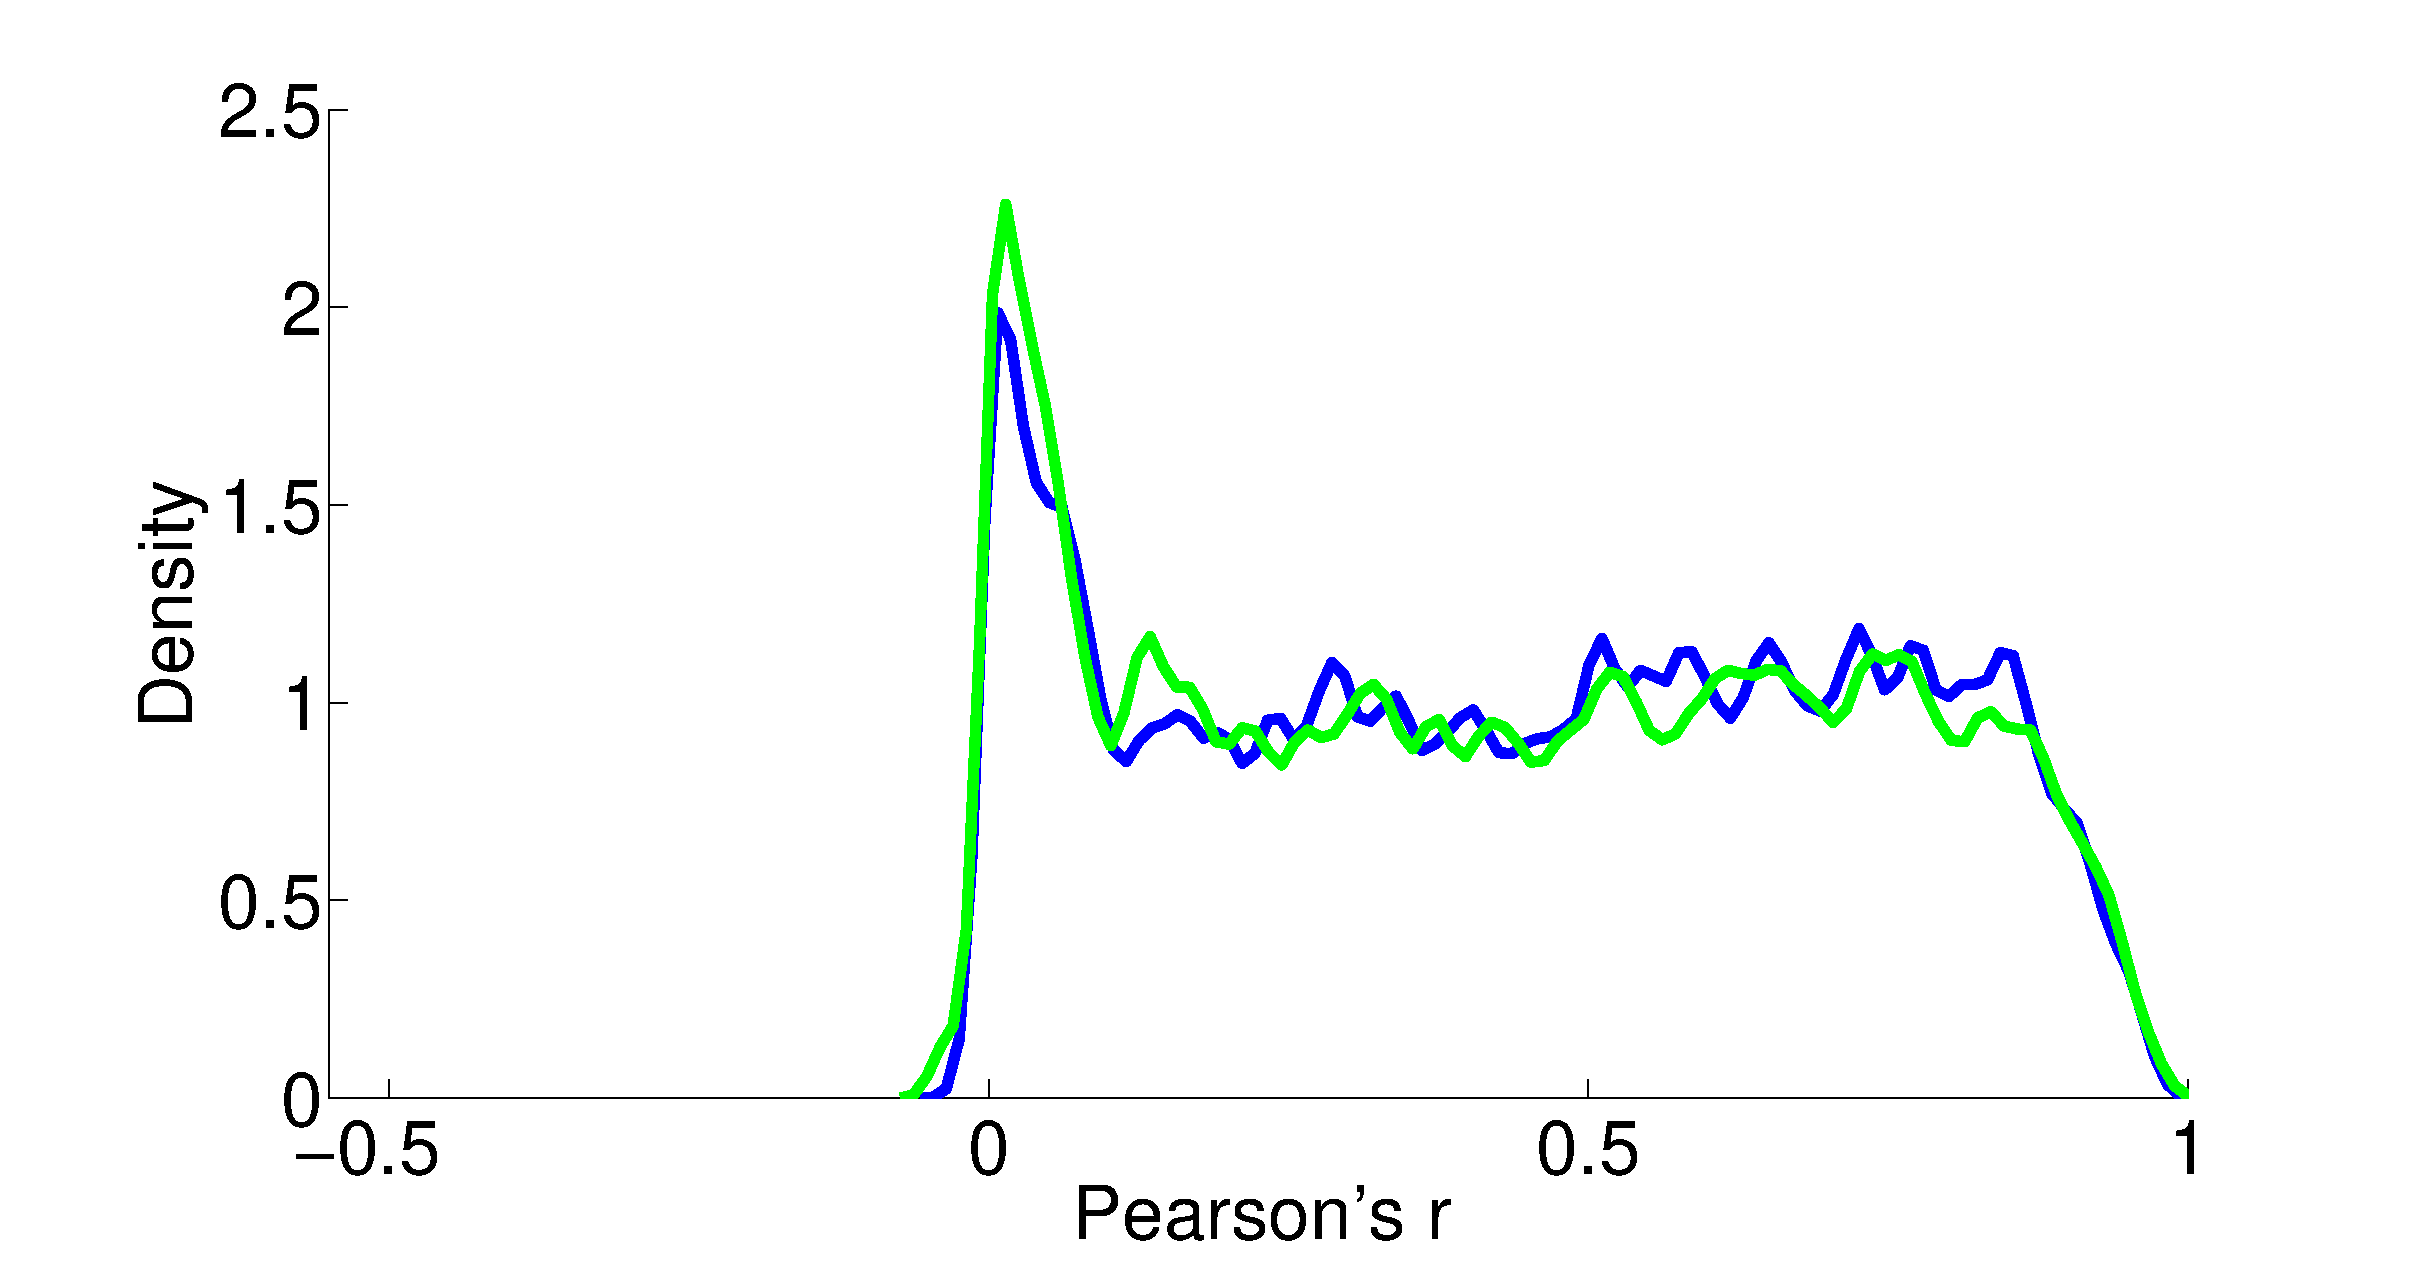
\includegraphics[width=\textwidth]{pFluxVec}
  \caption{highly constrained} \label{fig:YpermCorrSup:A}
  \end{subfigure}
&
  \begin{subfigure}[b]{0.5\textwidth}
  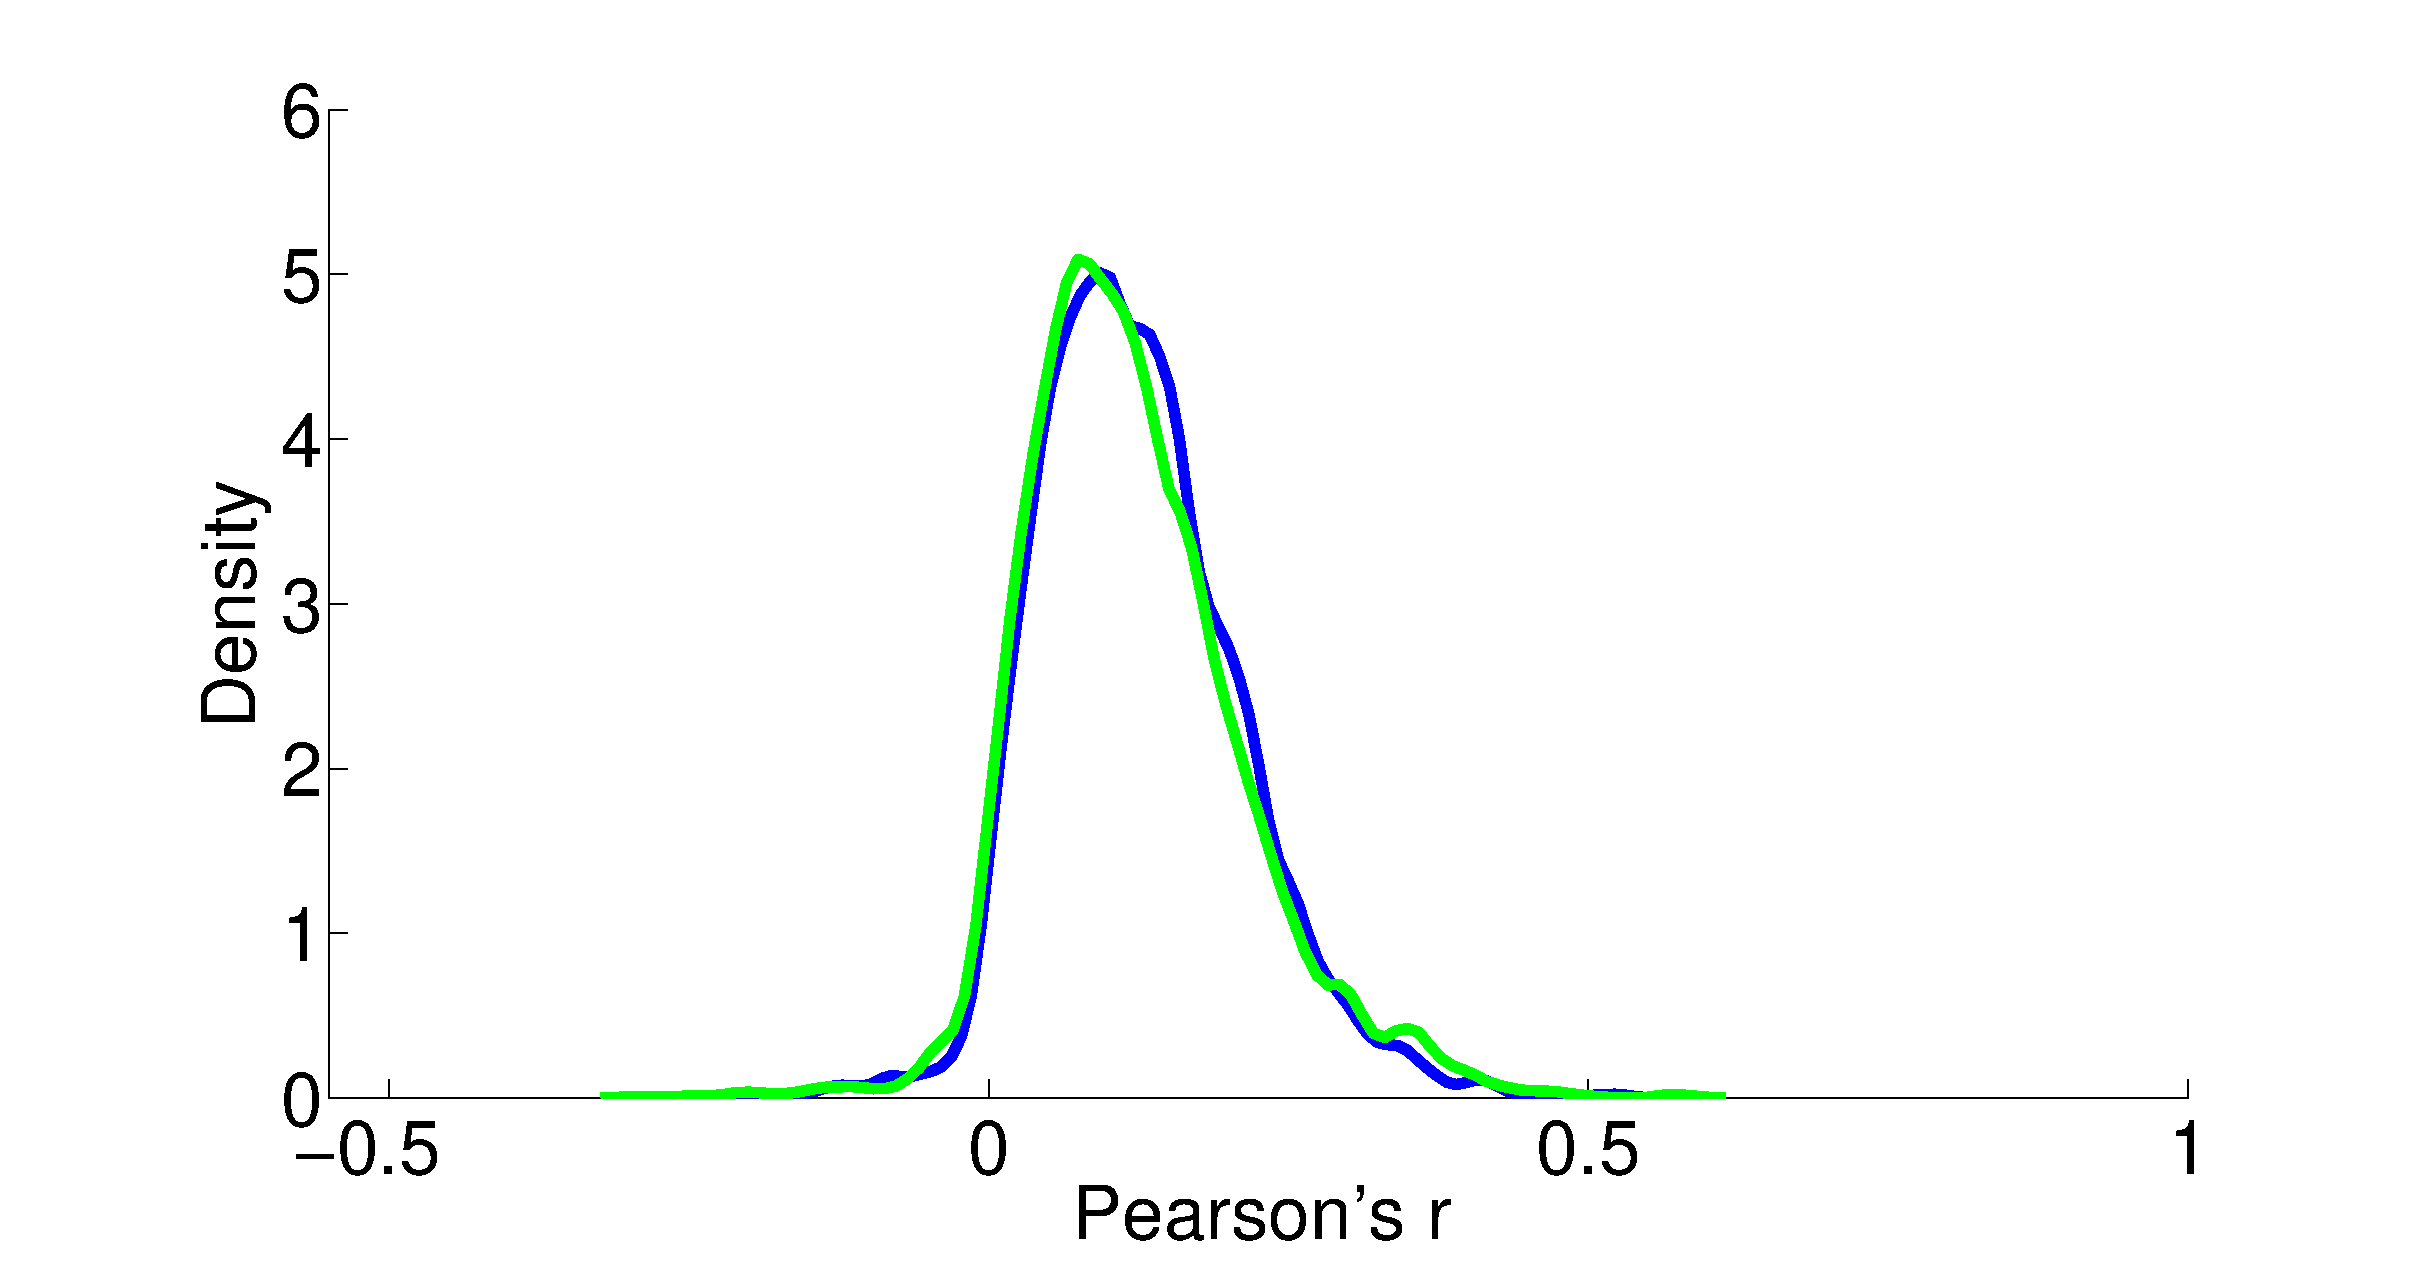
\includegraphics[width=\textwidth]{pFluxVec_dirr}
  \caption{minimally constrained} \label{fig:YpermCorrSup:B}
  \end{subfigure} 
\\
\end{tabular}
\vspace{-4mm}
\caption{PDFs of Pearson's correlation between fluxes estimated from
permuted and unpermuted complex abundance.}
\label{fig:YpermCorrSup:pearson}
\end{figure}
}

%%%%%%%%%%%%%%%%%%%%%%%%%%%%%%%%%%%%%%%%%%%%%%%%%%%%%%%%%%%%%%%%%%%%%%%%%%%%%%%%%%%%%%%%%%

\frame{\frametitle{Global flux correlations from permuted inputs} 

\begin{figure}[!htb]
\centering
\begin{tabular}{cc}
  \begin{subfigure}[b]{0.5\textwidth}
  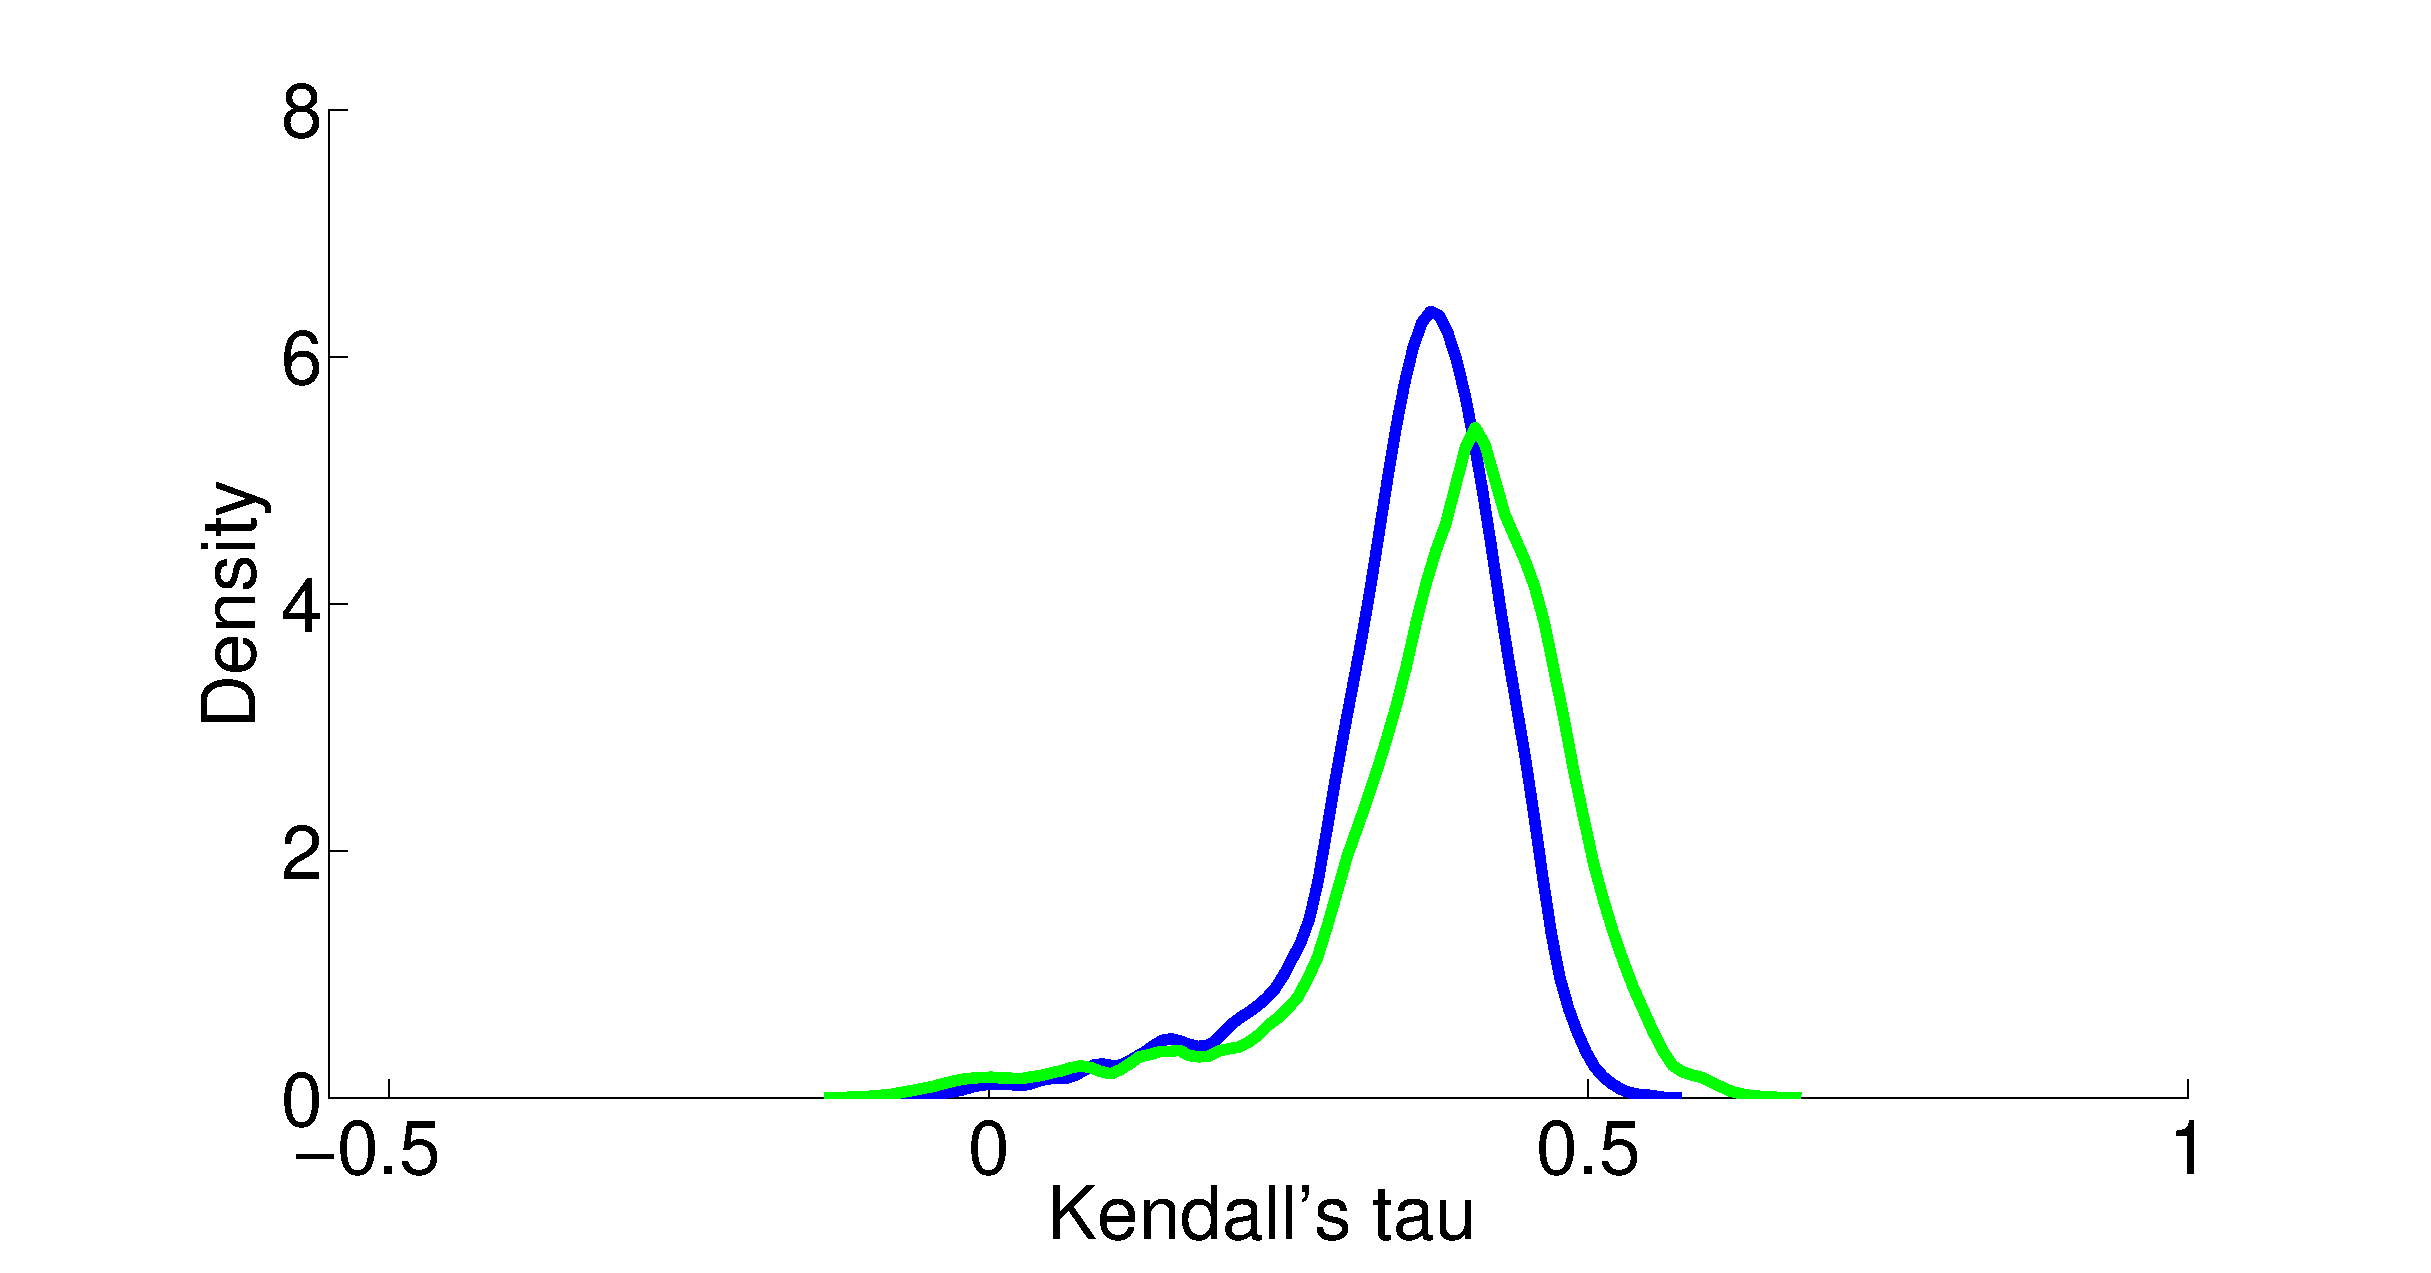
\includegraphics[width=\textwidth]{kFluxVec}
  \caption{highly constrained} \label{fig:YpermCorrSup:C}
  \end{subfigure}
&
  \begin{subfigure}[b]{0.5\textwidth}
  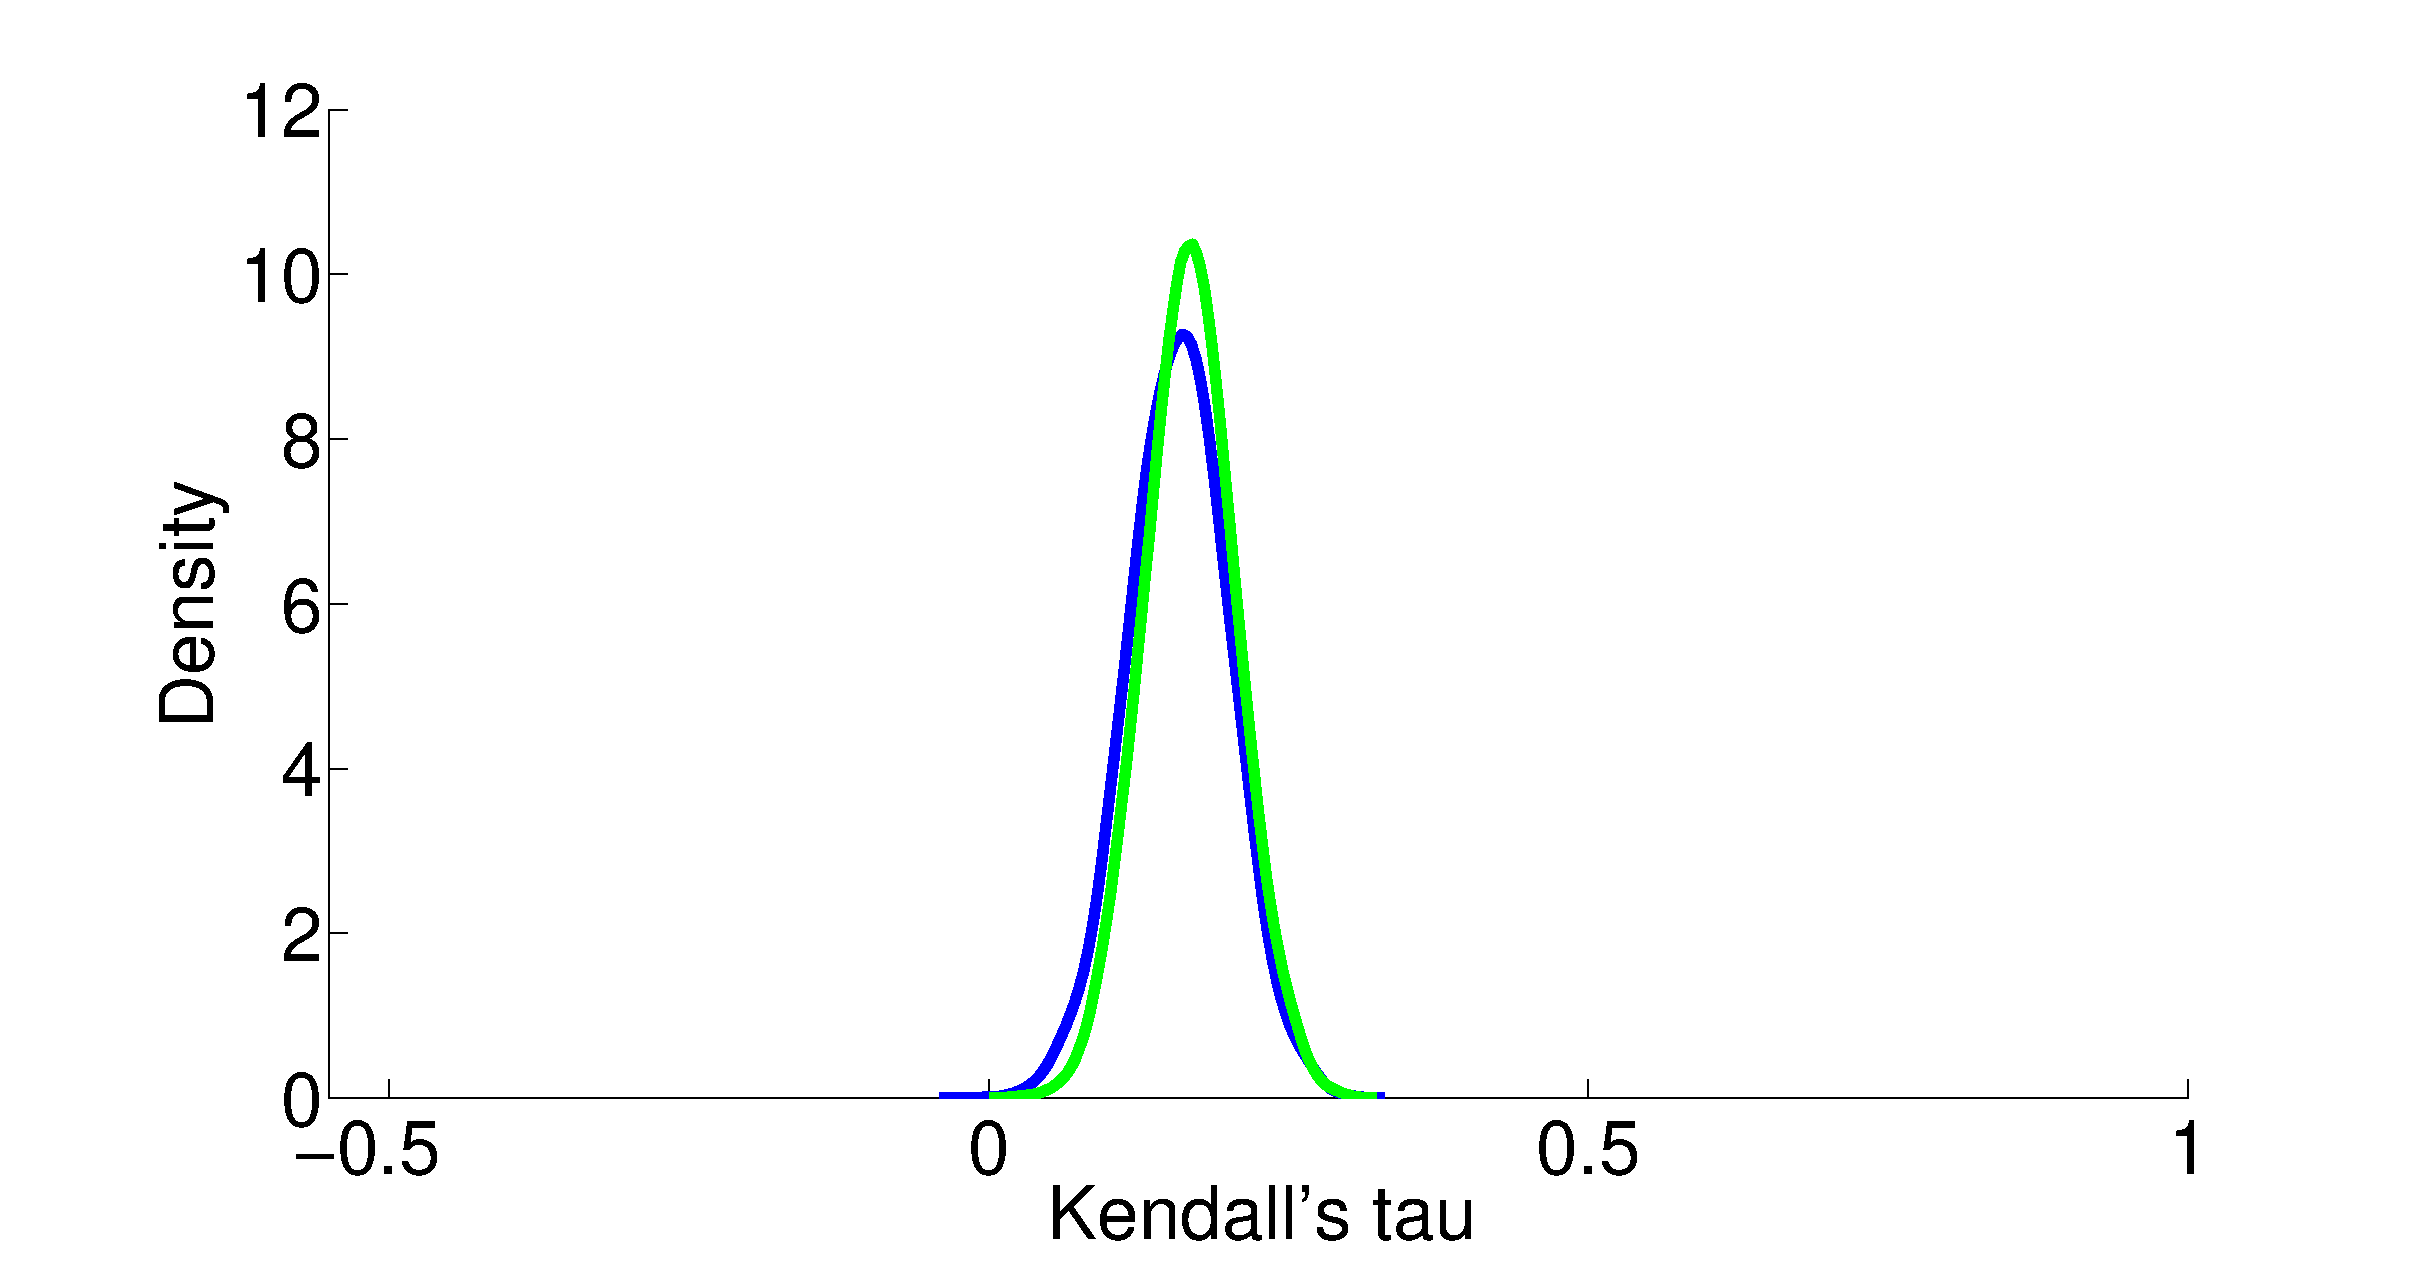
\includegraphics[width=\textwidth]{kFluxVec_dirr}
  \caption{minimally constrained} \label{fig:YpermCorrSup:D}
  \end{subfigure} 
\\
\end{tabular}
\vspace{-4mm}
\caption{PDFs of Kendall's correlation between fluxes estimated from
permuted and unpermuted complex abundance.}
\label{fig:YpermCorrSup:kendall}
\end{figure}
}

%%%%%%%%%%%%%%%%%%%%%%%%%%%%%%%%%%%%%%%%%%%%%%%%%%%%%%%%%%%%%%%%%%%%%%%%%%%%%%%%%%%%%%%%%%

\frame{\frametitle{Flux estimates give us more than just complex abundance} 

\hl{advantage of looking at flux over expression, which is commonly}
\hl{move this figure out and cite correlation}

\begin{figure}
\begin{tabular}{cc}
  \begin{subfigure}[b]{0.5\textwidth}   % l   b   r   t
  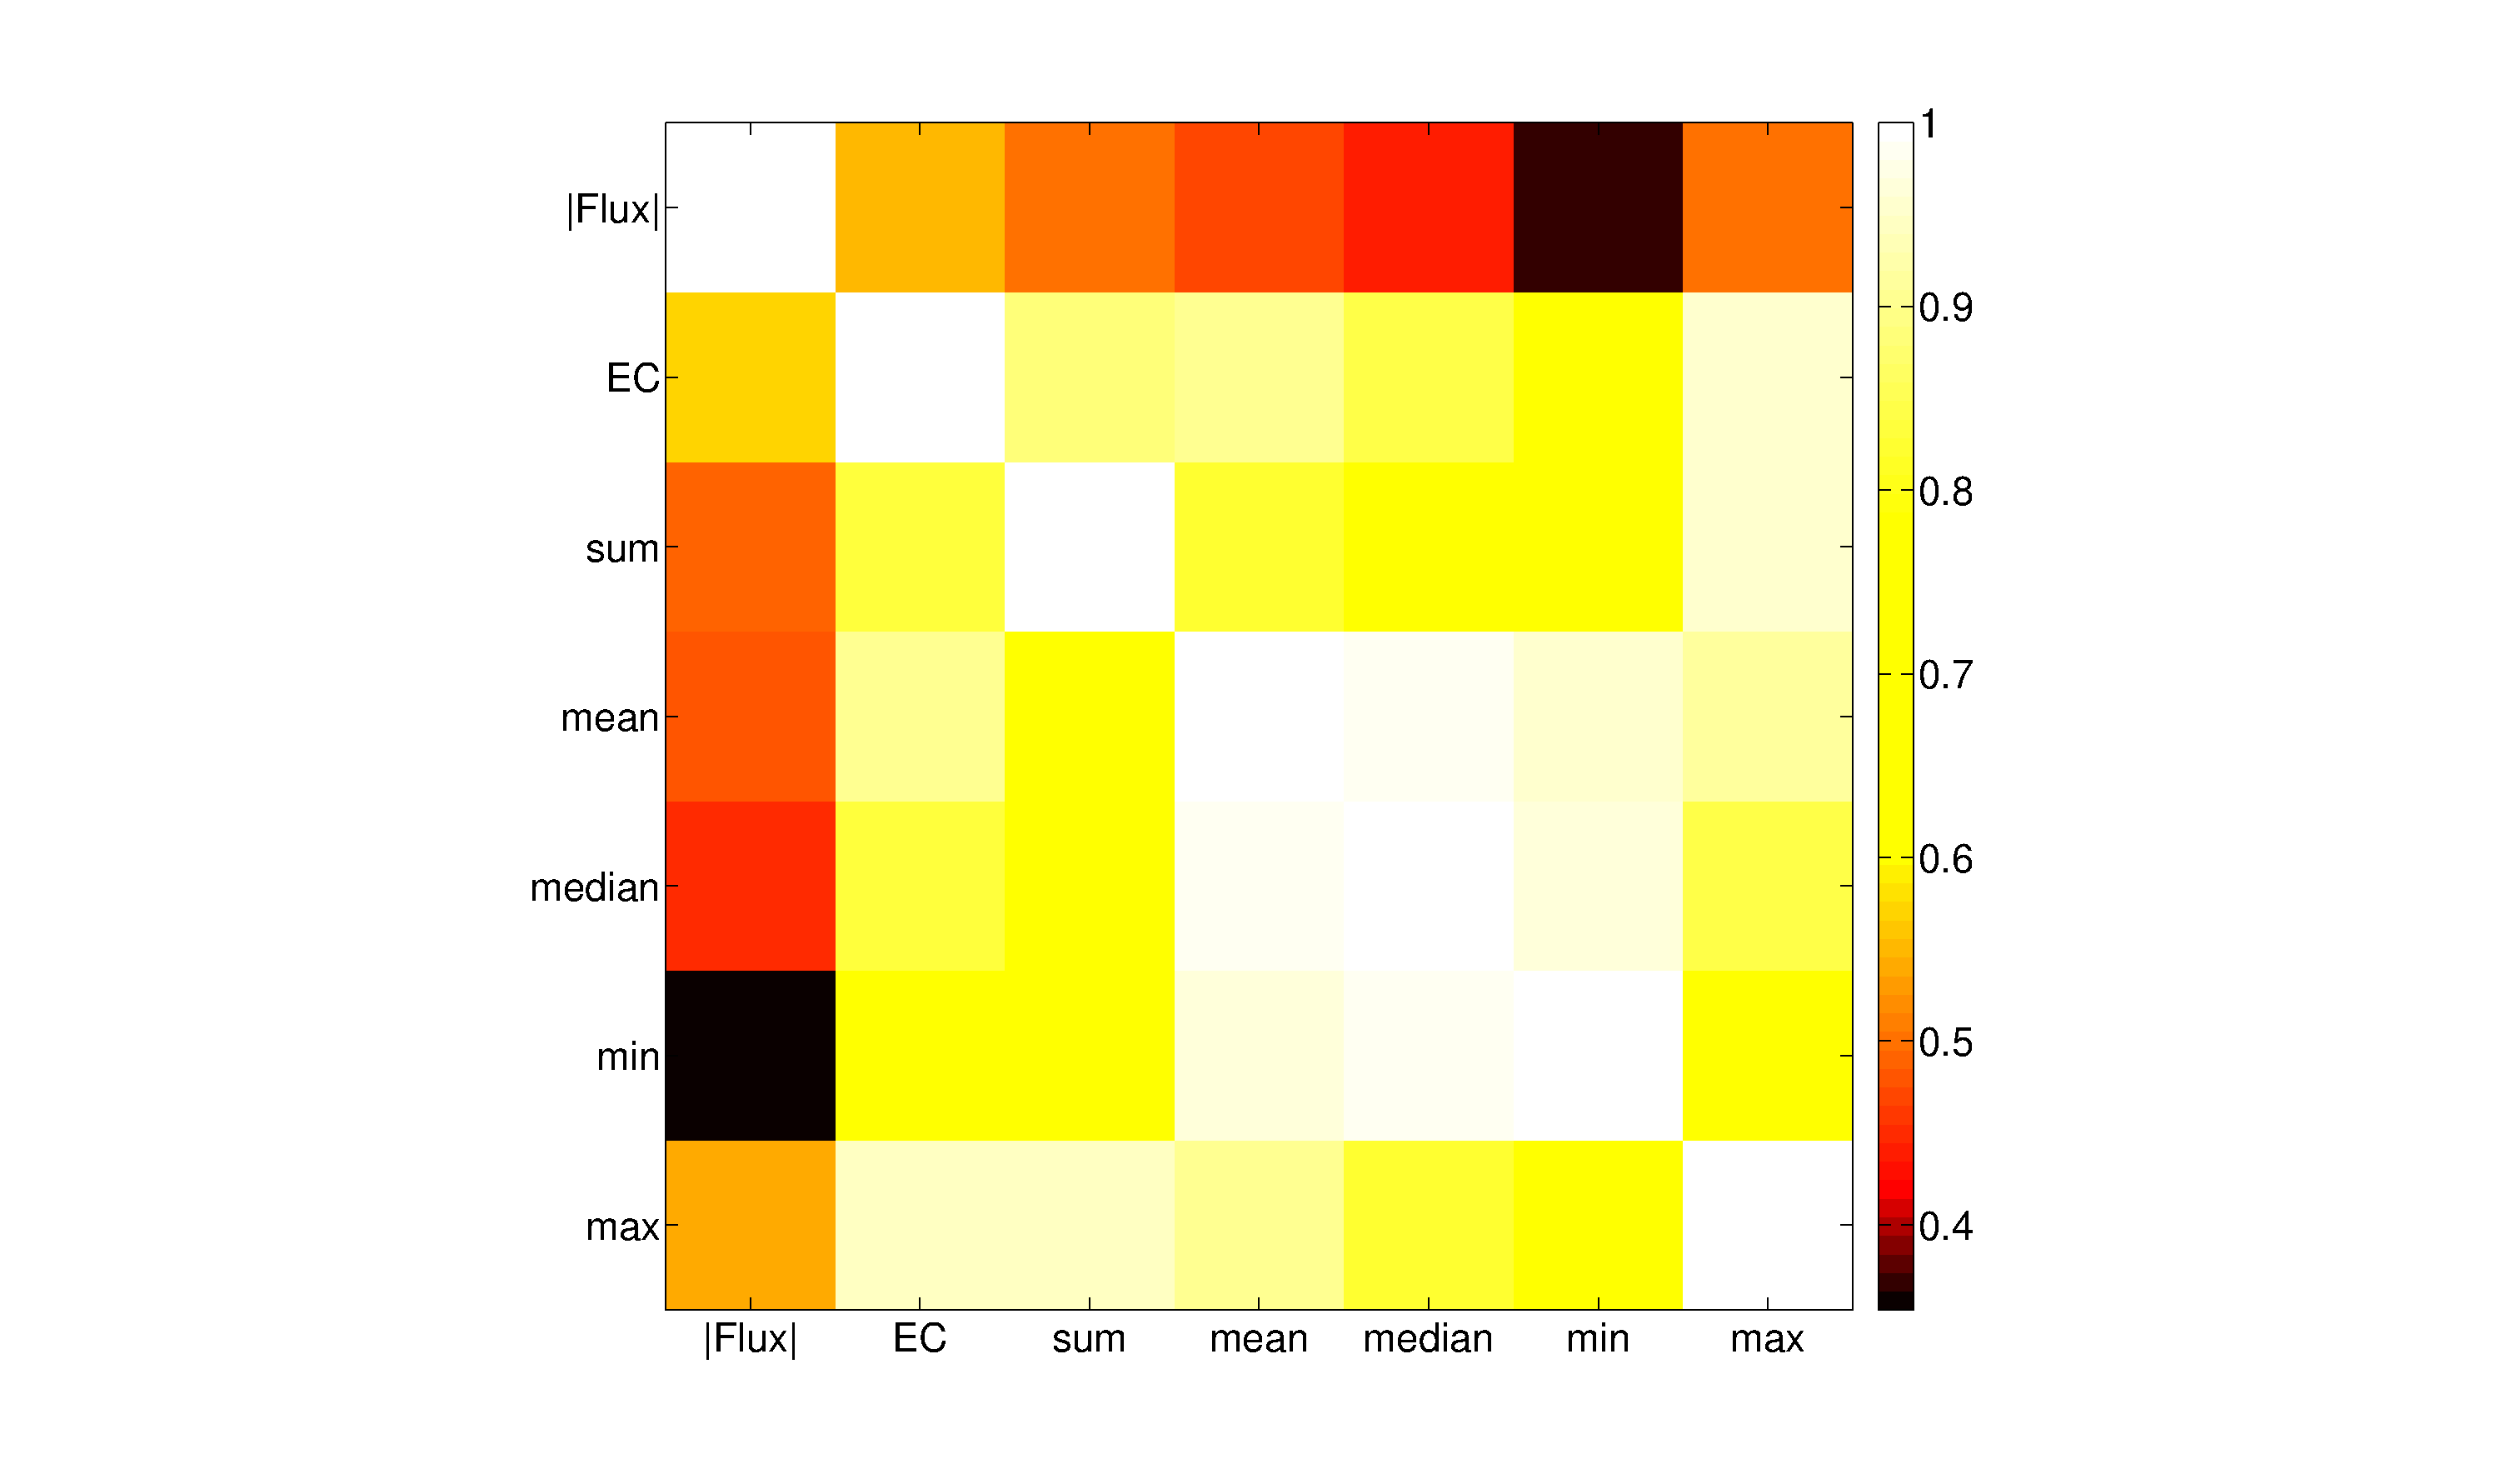
\includegraphics[width=\textwidth, trim=9cm 1.2cm 9cm 1cm, clip=true]
    {YeastExpFluxCompare}
  \caption{yeast} \label{fig:FluxExpCmp:A}
  \end{subfigure}
&
  \begin{subfigure}[b]{0.5\textwidth}
  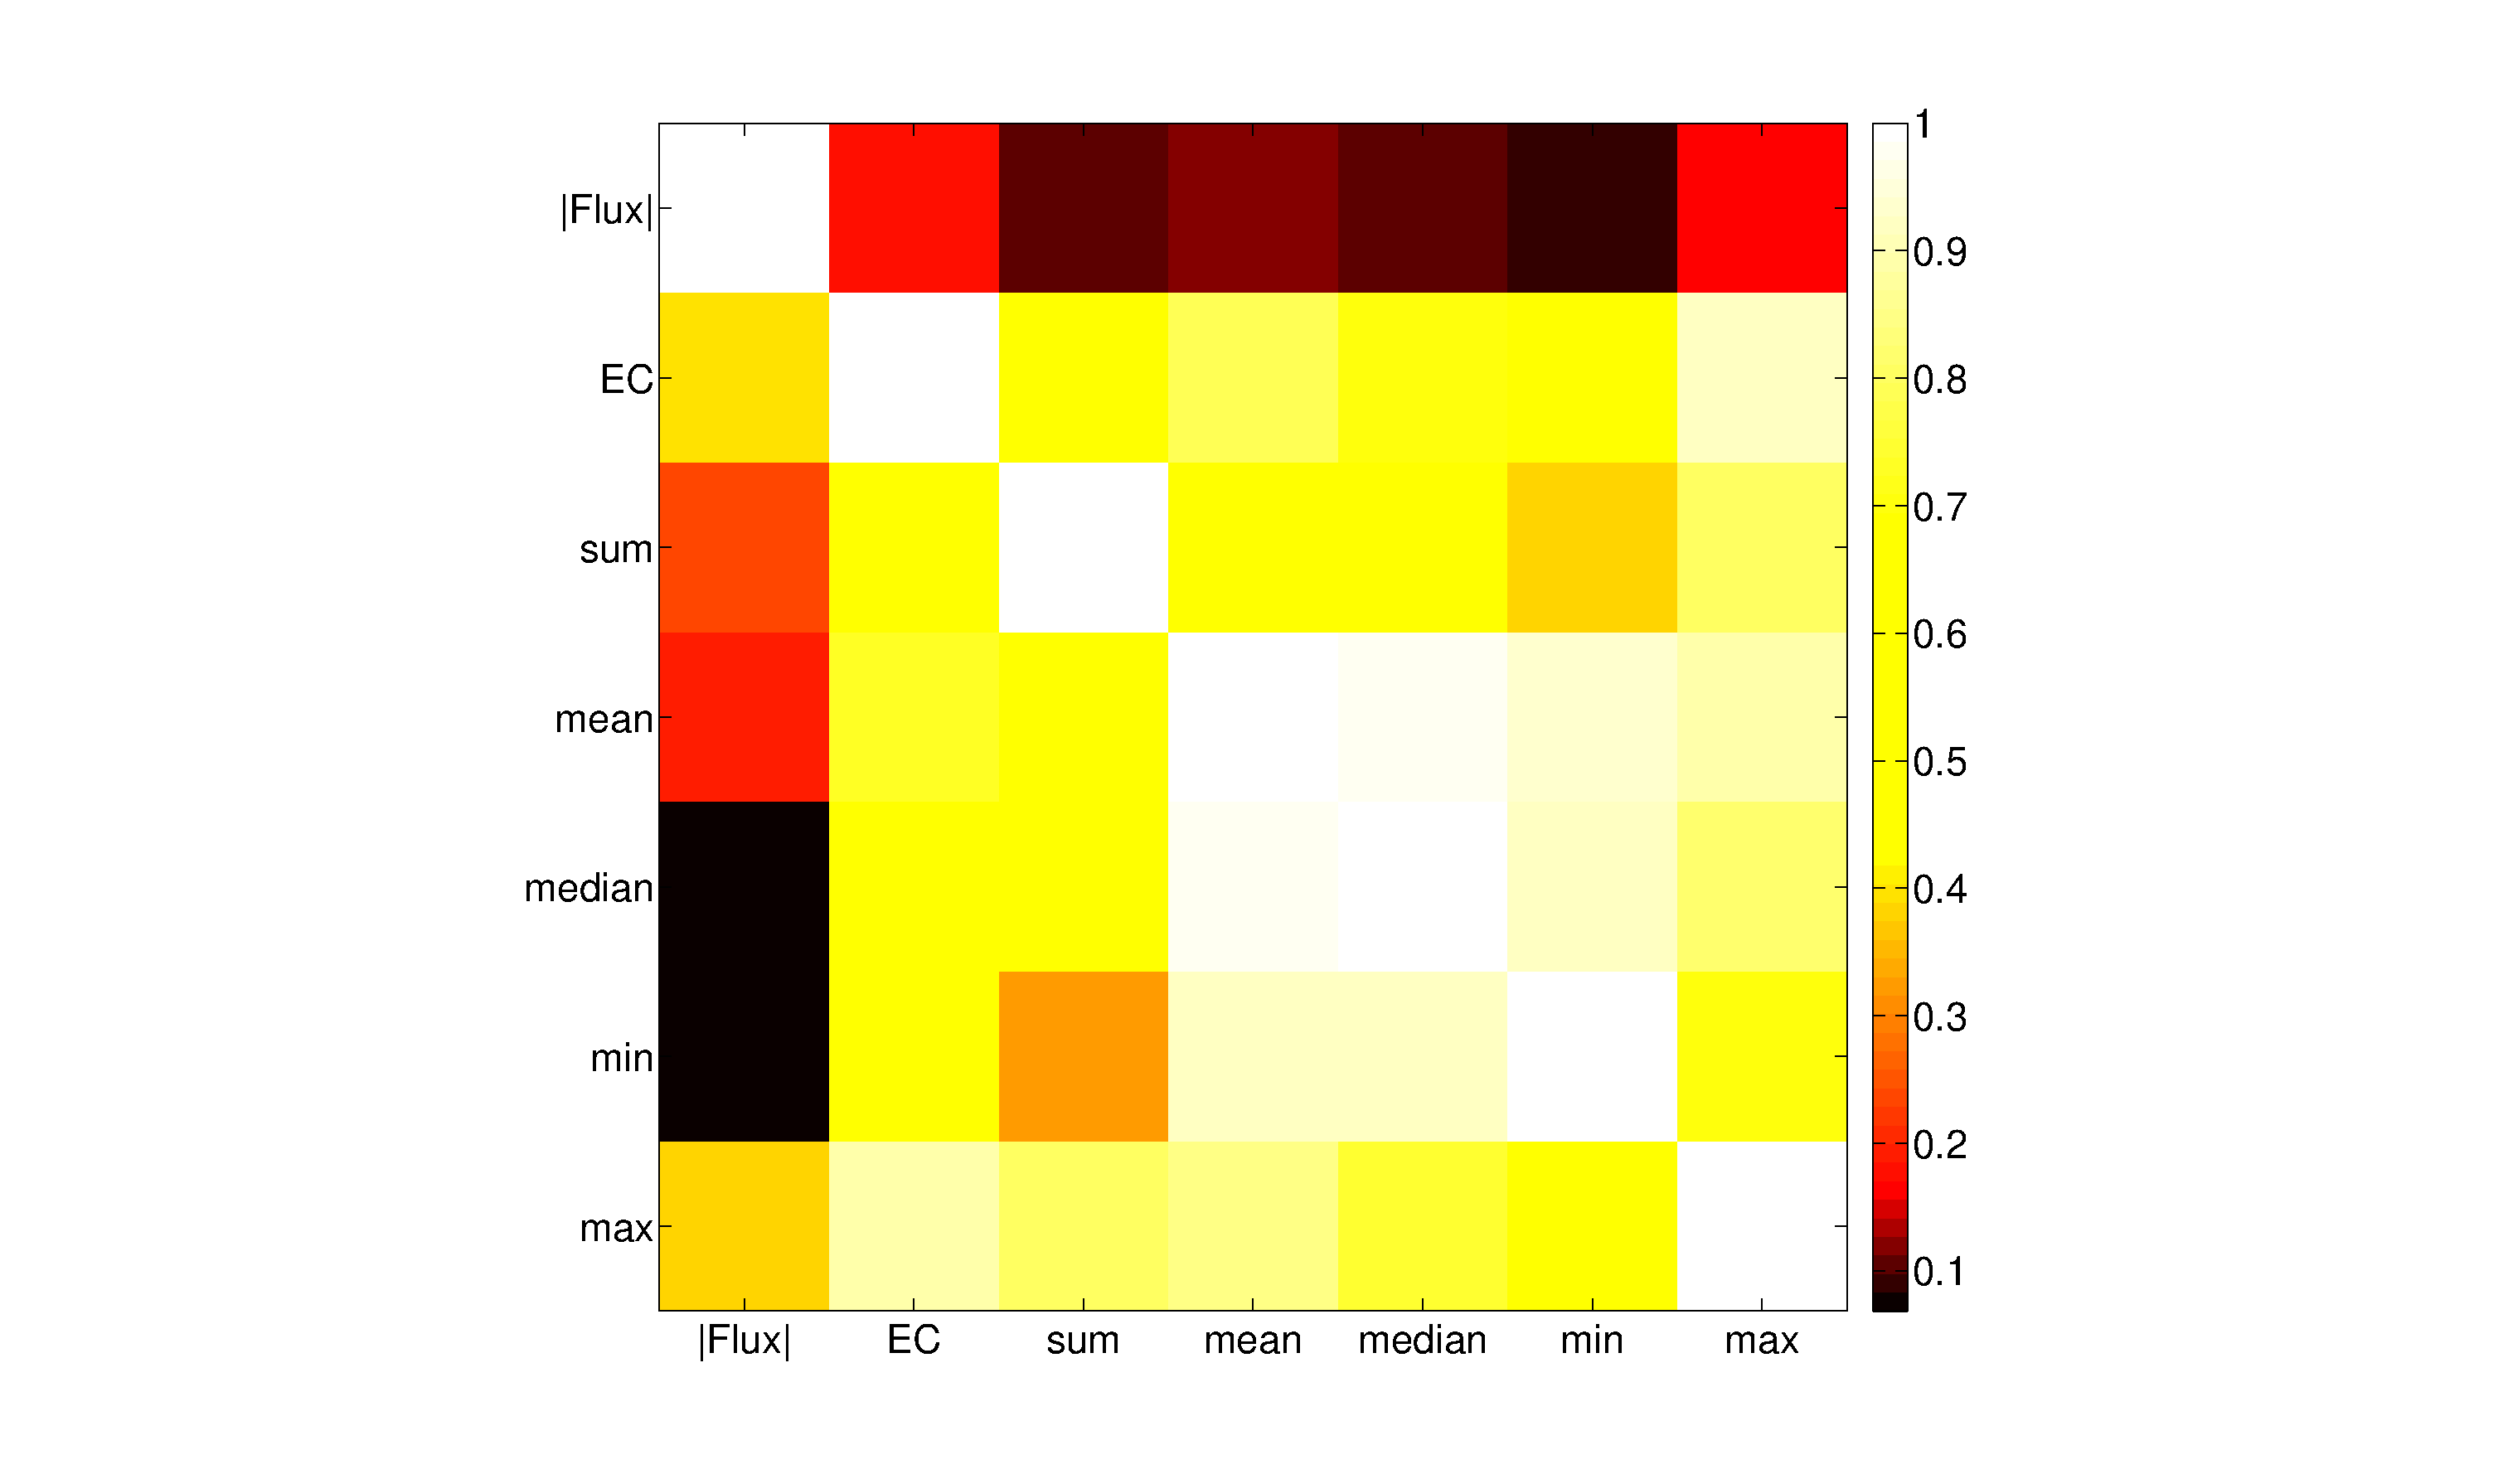
\includegraphics[width=\textwidth, trim=9cm 1.2cm 9cm 1cm, clip=true]
    {HumanExpFluxCompare}
  \caption{human} \label{fig:FluxExpCmp:B}
  \end{subfigure}
\\
\end{tabular}
\caption{Pearson correlation between FALCON flux magnitudes, and
various complexation estimates in yeast \textbf{(a)} and human
\textbf{(b)}.}
\label{fig:FluxExpCmp}
\end{figure}
}


%%%%%%%%%%%%%%%%%%%%%%%%%%%%%%%%%%%%%%%%%%%%%%%%%%%%%%%%%%%%%%%%%%%%%%%%%%%%%%%%%%%%%%%%%%
%%%%%%%%%%%%%%%%%%%%%%%%%%%%%% End Your Document %%%%%%%%%%%%%%%%%%%%%%%%%%%%%%%%%%%%%%%%%
%%%%%%%%%%%%%%%%%%%%%%%%%%%%%%%%%%%%%%%%%%%%%%%%%%%%%%%%%%%%%%%%%%%%%%%%%%%%%%%%%%%%%%%%%%

\end{document}

